% \documentclass[conference]{IEEEtran}
% \IEEEoverridecommandlockouts

% The preceding line is only needed to identify funding in the first footnote. If that is unneeded, please comment it out.
% \documentclass[11pt,dvipdfm,dvipsnames]{article}
\documentclass[11pt,dvipsnames]{article}
\usepackage{deauthor,times,graphicx}
\usepackage{cite}
\usepackage{amsmath,amssymb,amsfonts}
\usepackage{algorithmic}
\usepackage{textcomp}
% \usepackage{xcolor}
\usepackage{xcolor}

\usepackage{tcolorbox}
\usepackage{color}
\usepackage{cleveref}
\usepackage{booktabs} % For formal tables
\usepackage{bbding}

\usepackage{subcaption}

\usepackage{enumitem}
\setlist{nolistsep}
% \usepackage{hyperref}
\usepackage{pifont}
% \usepackage{natbib}
\usepackage{multirow,multicol}

\definecolor{cadmiumgreen}{rgb}{0.0, 0.42, 0.24}
\definecolor{cardinal}{rgb}{0.77, 0.12, 0.23}
\definecolor{cadmiumred}{rgb}{0.89, 0.0, 0.13}

\usepackage{fontenc}
\usepackage{inputenc}


\DeclareRobustCommand{\company}{Megagon Labs}%%

\newcommand{\code}[1]{\texttt{\small #1}}
\newcommand{\todo}[1]{\textcolor{red}{ #1}}

\newcommand{\nikita}[1]{\textcolor{blue}{\textbf{Nikita}: #1}}
\newcommand{\saj}[1]{\textcolor{magenta}{\textbf{Sajjadur}: #1}}
\newcommand{\dz}[1]{\textcolor{purple}{\textbf{Dan}: #1}}
\newcommand{\estevam}[1]{\textcolor{red}{\textbf{Estevam}: #1}}
\newcommand{\eser}[1]{\textcolor{orange}{\textbf{Eser}: #1}}

\newcommand{\eg}{{\itshape e.g.}, }
\newcommand{\ie}{{\itshape i.e.}, }

\newcommand{\stitle}[1]{\vspace{0.2em}\noindent\textbf{#1}}%%
\newcommand{\etitle}[1]{\vspace{0.2em}\noindent{{\it #1}}}%%
\newcommand{\emtitle}[1]{\vspace{0.15em}\noindent\underline{\em #1}}%%

\def\BibTeX{{\rm B\kern-.05em{\sc i\kern-.025em b}\kern-.08em
    T\kern-.1667em\lower.7ex\hbox{E}\kern-.125emX}}
\begin{document}

\title{Retrieval Augmented Generation in the Wild: A \emph{System 2} Perspective}

\author{Sajjadur Rahman\footnote{The first two authors contributed equally.} \quad Dan Zhang$^*$ \quad Nikita Bhutani \quad Estevam Hruschka \quad Eser Kandogan\\
Megagon Labs\\
\texttt{\{sajjadur, dan\_z, nikita, estevam, eser\}@megagon.ai}
}
% listed alphabetically by first name

\maketitle

\begin{abstract}
Large language models (LLMs), despite their impressive capabilities in natural language understanding tasks in open-domain, often lack effectiveness with similar tasks in enterprise applications due to potential hallucinations, weak multi-hop reasoning ability, and limitations in adapting to heterogeneous data types, among others. Such issues primarily arise due to the absence of private, on-premises enterprises from an LLM's training corpus. Knowledge-intensive tasks in enterprise often require multi-step reasoning, deep contextual understanding, and integration of information stored and accessed in heterogeneous formats (\eg tables, graphs, documents, and JSON), which LLMs aren't inherently equipped to handle without significant adaptation.
To this end, retrieval augmented generation (RAG) offers promise in instrumenting such adaptations on demand. 
While RAG-based approaches focus on controlling the generation and mitigating hallucinations, existing solutions are not sufficient for the requirements of the enterprise settings. 

In this paper, we outline our approaches toward understanding and implementing a more effective RAG workflow in the wild. To achieve the goal, we draw on the cognitive science concepts of System 1 (fast, intuitive thinking) and System 2 (slow, deliberate, analytical thinking.) In particular, we discuss how existing RAG approaches are more aligned to \emph{System 1} and propose to shift from traditional single-model architectures to compound AI systems within a \emph{System 2} framework to improve RAG, especially in complex enterprise applications. 
Such compound AI systems adopt a more systematic approach by assigning specialized tasks to different intelligent agents, optimizing retrieval and generation performance with a retrieval-augmented generation workflow. 
\end{abstract}


\section{Introduction}

Large Language Models (LLMs), despite their impressive performance across various natural language understanding tasks, exhibit significant limitations when applied to enterprise applications in the wild.
Primarily, these models may hallucinate—generating plausible-sounding but factually incorrect content—when their parametric knowledge does not align with specific enterprise data~\cite{maynez2020faithfulness,semnani2023wikichat,feng2024cmdbench}
. An LLM's parametric knowledge depends on its pre-training corpus and can also be influenced by the chosen training strategy and model architecture. This gap is especially problematic since enterprise applications frequently use private, on-premises data, which may differ substantially from the domains in LLMs' pre-training corpora.
Such domain misalignment can lead to severe inaccuracies, where the LLMs produce unreliable or misleading information.
%
In addition, enterprises often require consistency and reliability in their outputs. However, LLMs can be sensitive to prompt wording \cite{sclar2024quantifying}, producing inconsistent results even with minor phrasing changes, which undermines their reliability in high-stakes enterprise tasks.


Another key challenge for LLMs in enterprise settings is their limited capacity for complex reasoning. Many tasks in this domain require multi-step reasoning, deep contextual understanding, and coherent integration across different data sources, models, and pipelines. LLMs are not inherently designed to manage such complexities without extensive, task-specific adaptation and external grounding. These limitations hinder adopting LLMs in enterprise fields where accuracy, consistency, and reasoning depth are critical, such as healthcare, legal, HR, and data-driven decision-making applications.



%
Several approaches can help mitigate these limitations, including controlled generation, fact-checking, and post-processing. Controlled generation seeks to constrain the outputs of LLMs by guiding the model toward more reliable responses through techniques such as prompt engineering~\cite{brown2020language,wei2022chain,sahoo2024systematic}, fine-tuning~\cite{houlsby2019parameter,qin2023towards}, and reinforcement learning from human feedback~\cite{ouyang2022training}.
Fact-checking~\cite{thorne-etal-2018-fever,aly2021feverous} involves verifying generated content against highly credible sources to ensure accuracy, with any identified inaccuracies filtered out or corrected during post-processing. 
Although these techniques offer improvements, they may still struggle with domain-specific challenges and rapidly evolving knowledge.
\begin{figure}[t!] 
  %\vspace{-10pt}
  \centering
  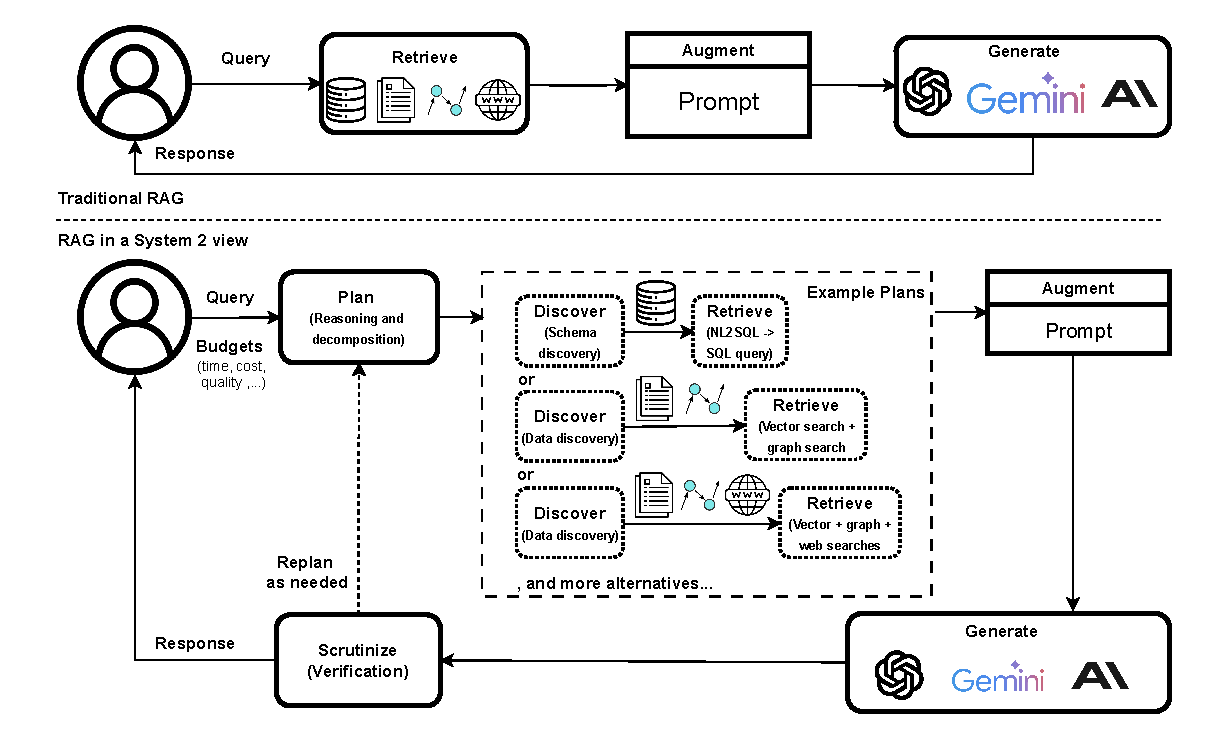
\includegraphics[width=\linewidth]{submissions/Estevam2024/figures/sys-rag2.pdf}
  \caption{Compared to the traditional RAG setup (above), where a fixed Retrieval-Augmentation-Generation workflow is executed, a System 2 approach (below) involves more deliberate reasoning and action based on critical analysis. For instance, given the same user query, the system must first plan by analyzing the task and may decide to decompose it into smaller components, such as data discovery, natural language-to-query translation, and actual query execution. During the planning phase, constraints or budgets related to factors like time, cost, or quality, along with the nature of the multimodal data sources, may influence the direction of the workflow. After the generation step, a verification process is typically required to evaluate the outcome, which may lead to revisions in subsequent iterations.}
  \label{fig:sys-rag2} 
\end{figure}
Among the various approaches, augmenting LLMs with external information sources has emerged as one of the most widely adopted solutions for enhancing accuracy and robustness. 
This strategy enables LLMs to access up-to-date, domain-specific knowledge, making them more adaptable to new fields or emerging topics. 
Techniques like retrieval-augmented generation (RAG)~\cite{lewis2020retrieval} integrate external databases or knowledge graphs to ground the model's outputs in verifiable information. 
By incorporating external data, such as multi-modal documents or enterprise-specific datasets, LLMs can produce more accurate and contextually relevant responses, thereby reducing the likelihood of hallucinations and making them more suitable for critical applications. However, simply using RAG approaches is not necessarily yet the definitive solution. Challenges remain, such as ensuring the quality and reliability of the retrieved information, handling ambiguous or conflicting data, and seamlessly integrating retrieval with generation to maintain coherent and contextually appropriate responses. Consequently, there is still considerable room for improvement in creating more robust and reliable AI systems.



As already shown in the literature, the idea of \emph{System 1} and \emph{System 2} \cite{kahneman_thinking_2012},  can be helpful to contextualize the current capabilities and limitations of LLMs \cite{bengio2019system}. In cognitive sciences, \emph{System 1} refers to fast, intuitive, and automatic thinking. This type of system can be characterized by fast thinking or quick judgments and decisions that rely on heuristics and subconscious processing. System 1 is highly efficient for everyday tasks that require intuitive, fast, unconscious, and immediate responses.
System 2, however, is associated with slow, deliberate, and analytical thinking. It is more helpful and used for complex problem-solving, critical analysis, and tasks that require conscious, sequential, algorithmic planning and reasoning. System 2 is more resource-intensive and slower but more reliable for tasks requiring careful consideration. 

In this System~1/System~2 context, we argue that even though RAG approaches have strong potential to contribute to reducing limitations of current LLMs (by playing a role more closely related to System 2), most current RAG approaches only weakly resemble System 2 thinking. The retrieval and generation steps are often designed to be fast and instantaneous, aligning with System 1 thinking, rather than slow and logical as in System 2, which presents challenges on both the data and model sides. For example, research \cite{maekawa-etal-2024-retrieval,ding2024retrieve} has shown that augmenting LLMs with retrieval without rigorously assessing necessity may adversely impact overall performance. 



Therefore, as illustrated in Figure~\ref{fig:sys-rag2}, we advocate for a shift from traditional single-model architectures to compound AI systems within a System 2 framework to enhance RAG, particularly in complex enterprise applications. Compound systems enable a collaborative approach to problem-solving by distributing specialized tasks across distinct agents, each optimized for specific functions, improving both retrieval and generation performance in challenging real-world settings.

On the retrieval side, enterprise applications often involve complex, multi-step, and sometimes ambiguous tasks that require deeper reasoning and structured workflows. A compound system can enhance this by assigning specialized agents to handle diverse aspects of data, such as heterogeneous formats (e.g., text, tables, graphs, parametric information) and noisy or incomplete data sources. This allows for agents skilled in reconciliation and semantic querying to refine the retrieval process through iterative, logic-driven interaction, improving both precision and relevance of context.

On the generation side, challenges like hallucination, fact verification, and adherence to context remain key obstacles. In a compound system setup, individual agents can be tasked with verifying facts, maintaining context alignment, and evaluating outputs for accuracy before finalizing responses. This division of labor can be exploited towards reducing hallucinations and enhancing reliability by enabling dynamic inter-agent evaluation, where each agent iteratively cross-checks and validates the others' outputs \cite{zhang2021survey,carlson2010toward}. For example, in domain-specific conversational AI, particularly in regulated industries, compound AI systems offer a pathway to safer, more reliable, and robust deployments by integrating domain expertise, context sensitivity, and rigorous validation at each step. 


The paper is organized as follows. First, in \cref{sec:background}, we provide a brief overview of traditional RAG models and highlight their limitations, especially in real-world, domain-specific applications. We then motivate more concretely the need for a System 2 RAG approach, in section 3. In \cref{sec:sys2}, several approaches to enhance RAG adaptability to System 2 thinking are discussed. Finally, we present our vision for future research in \cref{sec:future}, exploring the potential of compound AI systems as System 2 solutions to RAG.


\section{Background}
\label{sec:background}

\subsection{Traditional Approaches Towards RAG}
Retrieval augmented generation (RAG) aims to address hallucinations and factual inaccuracies in LLM-generated content. RAG infuses 
external knowledge~\cite{peng2023check, lazaridou2022internet}, such as knowledge bases and web documents, while prompting LLMs to help generate responses grounded on relevant information. The integration of RAG-based workflows in prompting LLMs has enjoyed widespread adoption, enhancing the suitability of LLMs for real-world applications. Development of a RAG system often begins with an indexing step, which involves cleaning and segmenting the documents --- segmentation is required to prepare chunks of information that carry meaningful and strong signals, and in addition, to fit into an LLM's context window (when using LLMs with limited context windows). Each chunk is then encoded into a vector representation using an embedding model and stored in a vector database. This step is essential for enabling efficient similarity searches in the subsequent retrieval phase. As shown in Figure~\ref{fig:sys-rag2}, the following are the standard phases of a traditional RAG workflow:

\stitle{Retrieval.} Given a user query, a RAG system employs an encoding model used during indexing to transform the query into a vector representation and calculates the similarity scores between two vectors: query and candidate text chunks within the indexed corpus. Based on these scores, the system retrieves the top-$K$ chunks with the highest similarity to the query, which are then used as the expanded context for the next stage.

\stitle{Augmentation.} The selected chunks are incorporated into a prompt as expanded context to provide additional relevant information. The goal of such enhancement is to reduce hallucination and improve accuracy of the model’s response. By providing targeted context, the RAG system ensures the model can ground its answer in the most pertinent retrieved data.

\stitle{Generation.} The user query, along with the augmented context of selected documents, is synthesized into a coherent prompt, which is then provided to an LLM that will perform the final generation task. Depending on the task requirements, the model may either draw upon its internal knowledge or limit its response to information in the provided documents. 

\subsection{Limitations of RAGs}

Traditional approaches to RAG do not directly apply to real-world scenarios due to the heterogeneity of data, the complexity of workflows, and the strict constraints on expected task performances.

\subsubsection{Lack of Robust Deliberation}

\newcommand{\crimson}{red}
\newcommand{\darkgreen}{green}

\begin{table*}[!htb]
    \centering
    \scriptsize
    % \resizebox{\textwidth}{!}{
    \begin{tabular}{p{15.5cm}}
        \toprule
        \textbf{Triple: }(Chicago, country, United States of America) \hfill \textbf{Entity Popularity: $95.0\%ile$}\\
        \textbf{Question:} What country is Chicago located in? \hfill\textbf{Entity-Relation Popularity: $97.4\%ile$}\\ %  Popular + no retrieval error\\
        \textbf{LM Answer:} United States {\color{\darkgreen}[Correct]}\\
        \textbf{Context: } The Chicago Municipal Tuberculosis Sanitarium was located in Chicago, Illinois, USA.\dots{\color{\darkgreen}[Correct Retrieval]}\\
        \textbf{RALM Answer:} USA {\color{\darkgreen}[Correct]}\\\midrule
        \textbf{Triple: }(George H.W. Bush, educated at, Yale University) \hfill \textbf{Entity Popularity: $89.5\%ile$}\\
        \textbf{Question:} What educational institution did George H.W. Bush attend? \hfill \textbf{Entity-Relation Popularity: $41.8\%ile$}\\% Popular + retrieval error\\
        \textbf{LM Answer:} Yale University {\color{\darkgreen}[Correct]}\\
        \textbf{Context: } The George H.W. Bush Presidential Library is located on a site on the west campus of Texas A\&M University in College Station, Texas.\dots {\color{\crimson}[Wrong Retrieval]}\\
        \textbf{RALM Answer:} Texas A\&M University {\color{\crimson}[Wrong]}\\\midrule
        \textbf{Triple: }(Ellen Litman, educated at, University of Pittsburgh) \hfill \textbf{Entity Popularity: $10.3\%ile$}\\
        \textbf{Question:} What educational institution was Ellen Litman educated at? \hfill \textbf{Entity-Relation Popularity: $17.9\%ile$} \\ % Less Popular + no retrieval error\\
        \textbf{LM Answer:} Stanford University {\color{\crimson}[Wrong]} \\
        \textbf{Context: } Ellen Litman Ellen Litman (born 1973) is an American novelist. She received the Rona Jaffe Foundation Writers' Award in 2006. Born in Moscow, Russia, she emigrated with her parents in 1992 to Pittsburgh, Pennsylvania. She was educated at the University of Pittsburgh and earned a B.S. in Information Science. \dots{\color{\darkgreen}[Correct Retrieval]}\\
        \textbf{RALM Answer:} University of Pittsburgh {\color{\darkgreen}[Correct]}\\\bottomrule
    \end{tabular}
    \vspace{-2mm}
    \caption{QA examples from WiTQA with predictions of varying popularity of question entity and entity-relation pair. The predictions from LM (GPT-3.5) with no augmentation and RALM (GPT-3.5+BM25) are shown. In the top row, both LM and RALM provide correct answers for the popular question. In the middle row, LM generates correct answer but RALM provides incorrect answer due to retrieval errors. In the bottom row, LM provides incorrect answer for an infrequent entity-relation pair.
    }
    \vspace{-3mm}
    \label{tab:example_adaptive_retrieval}    
\end{table*}

Recent studies show how RAGs are not universally effective~\cite{petroni-2020,li-etal-2023-large}. Adding noisy or irrelevant passages can override correct LM knowledge, leading to errors (see Table \ref{tab:example_adaptive_retrieval}). An effective RAG should balance accurate recall with selective retrieval. Identifying when to recall versus retrieve raises key questions: (a) What factors impact an LM’s recall accuracy? (b) What influences RAG performance? (c) What error patterns are common between LM and retriever responses?


Previous research on memorization in LMs and retriever performance has some limitations: (a) it focuses only on entities, while real-world information includes both entities and relations~\cite{sun2023headtotail,mallen-etal-2023-trust}. (b) It examines either retrievers or LM recall independently, overlooking their interplay~\cite{petroni-etal-2019-language, sciavolino-etal-2021-simple,liu2023pre}. To address these limitations, in previous work, \cite{maekawa-etal-2024-retrieval} focused on the QA task and analyzed the performance of 10 LMs across 5 retrieval settings. They introduced \textsc{WiTQA} \cite{maekawa-etal-2024-retrieval}, a new dataset of QA pairs generated from Wikipedia triples, selected based on entity and relation popularity, each paired with supporting passages and popularity scores. The investigation of RAGs zero-shot performance on \textsc{WiTQA} yields the following key findings (see Figure \ref{fg:head_tail_vanilla}):

\begin{figure}[th!]
    \centering
    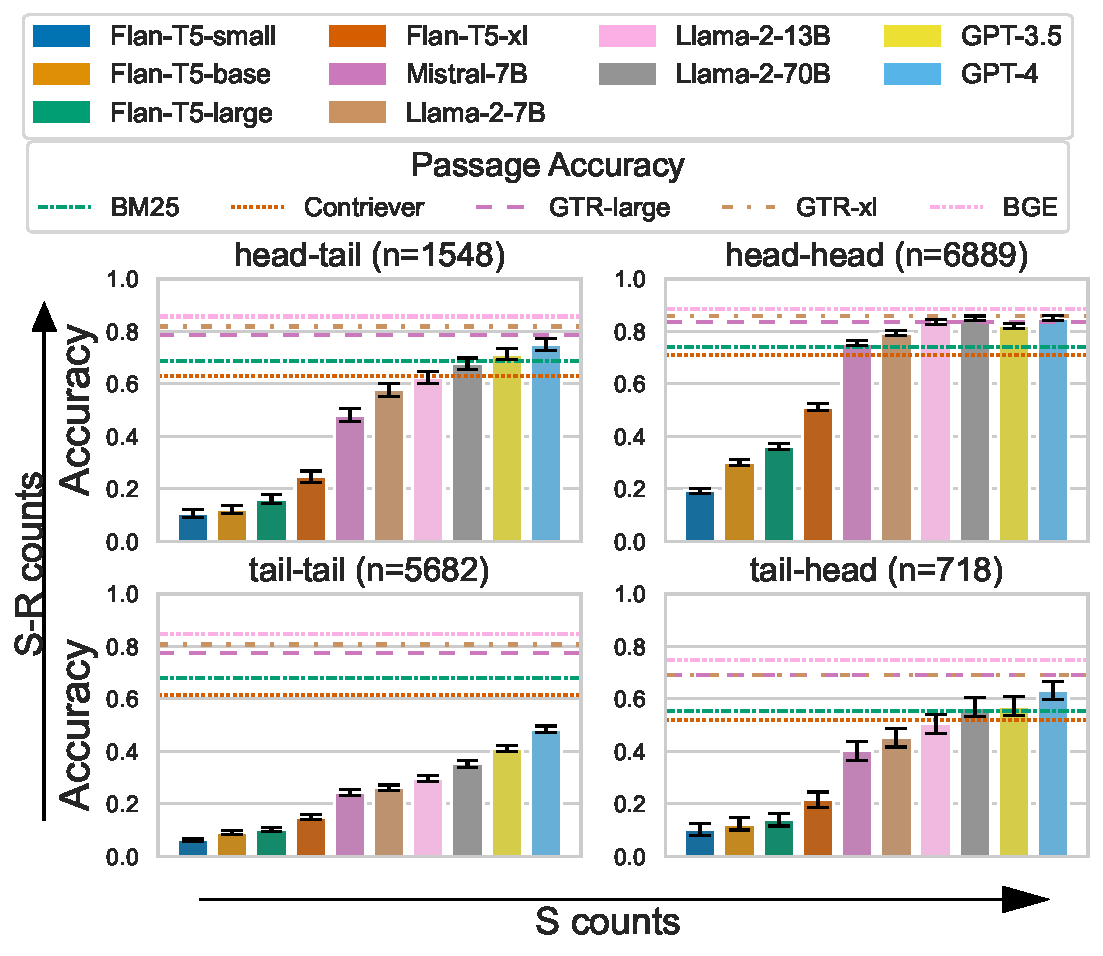
\includegraphics[width=0.48\textwidth]{submissions/Estevam2024/figures/head_tail_witqa200_for_vanilla_gtr.pdf}
    \caption{Analysis on Vanilla LMs with BM25, Contriver, GTR, and BGE passage accuracy over S-R counts and S counts ($n=$ the number of questions in the group). In the top row, S-R counts are higher than the median. In the bottom row, they are less than or equal to the median. In the left column, S counts are less than or equal to the median, and in the right column, they are higher than the median.} 
    \label{fg:head_tail_vanilla}
\end{figure}

\begin{itemize}
    \item LMs can often recall frequently encountered entity-relation pairs from pre-training without retrieval, but this depends on model size; larger models capture more long-tail relations for popular entities, though accuracy drops for less common facts.
    \item For long-tail entity-relation pairs, retrieval performs better than LM recall, suggesting retrieval augmentation benefits these cases but may introduce override issues with well-known pairs.
    \item LMs outperform retrievers on well-known entity-relation pairs involving long-tail entities, contrasting prior studies where large LMs struggled with these pairs.
\end{itemize}

\noindent
Using these insights, a selective memory integration module was designed, that applies retrieval augmentation or LM recall based on entity-relation popularity. The main idea is closely related to a System 2 approach, in which before trying to answer a question, the system first tries to figure out (reasoning task) whether it should use the retrieval mechanism or not.  It was found it could improve QA performance by up to 10.1\% \cite{maekawa-etal-2024-retrieval}.

%% Text Operators
Another limitation of most current RAG models is characterized by their reliance on localized context retrieval, making them less effective for tasks that require \textit{holistic reasoning}—the ability to synthesize, aggregate, and analyze information across multiple documents. For instance, when asked, ``Which company employed the most people?'' traditional retrieval models may return individual statistics for each company without a comprehensive comparison. This core limitation reveals that while RAG systems are adept at fact retrieval, they falter with broader, cross-document reasoning. Bridging this gap requires models capable of multi-document synthesis, comparative analysis, and extensive dataset integration.

One alternative to to address these limitations of RAG models in holistic reasoning is to bypass retrieval altogether and use long-context language models (LCLMs).  These models are designed to handle and process significantly larger chunks of information, enabling them to reason effectively over extensive contexts or large sets of documents without the need for iterative retrieval steps. By eliminating the dependency on retrieval mechanisms, LCLMs reduce the risk of retrieving irrelevant or incomplete information, which can compromise reasoning quality. Furthermore, their ability to maintain coherence across lengthy inputs makes them particularly well-suited for tasks requiring nuanced understanding, cross-referencing of details, and synthesis of insights from diverse sources within a single reasoning framework.

To investigate into this, \cite{maekawa2024holistic} conducted a comparative study of LCLMs and RAG models using HoloBench, a benchmark specifically designed to evaluate holistic reasoning capabilities. It compared two large LCLMs, Llama-3.1-405b and GPT-4o, alongside a smaller LCLM, Llama-3.1-8b. For document retrieval, the work employed \texttt{\small BAAI/bge-large-en-v1.5}, an effective embedding-based model that retrieves the 2k tokens most similar to the query.

The findings in \cite{maekawa2024holistic}  reveal that as context length exceeds 4k tokens, larger vanilla LCLMs consistently outperform RAG-based models, indicating their superior ability to manage longer contexts where RAGs struggle to retrieve relevant information (see Figure ~\ref{fig:rag}). Interestingly, with smaller models like Llama-3.1-8b, RAG performs better when context length surpasses 16k tokens. This aligns with previous findings\cite{maekawa-etal-2024-retrieval} that retrieval models can enhance the performance of weaker models by compensating for their reasoning limitations, even in the presence of retrieval errors. A promising future direction would be to adopt a System 2-based approach and integrate a dynamic mechanism for determining the optimal amount of information to retrieve based on the query and context length, particularly when working with weaker models for holistic reasoning.

\begin{figure}[ht]
    \centering
    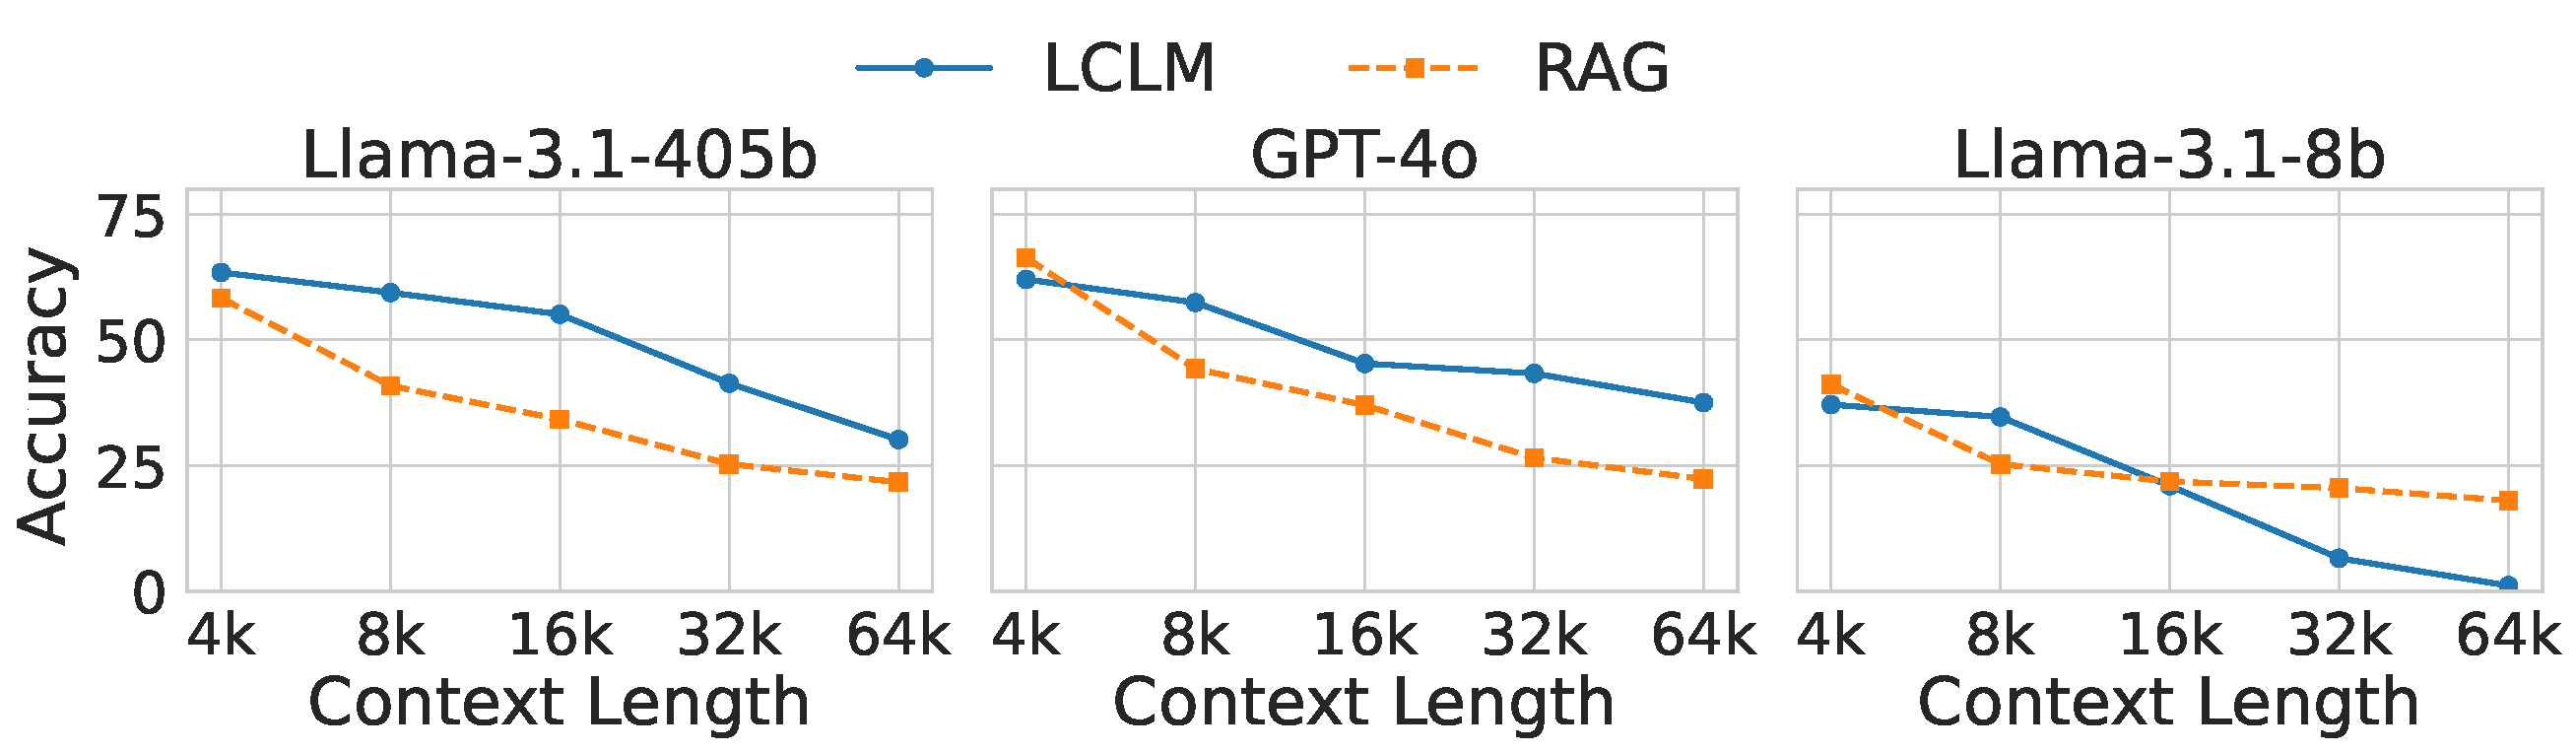
\includegraphics[width=.8\linewidth]{submissions/Estevam2024/figures/lclm_vs_rag_all_models.pdf}
    \caption{Performance comparison of LCLM and RAG. For long contexts, large models outperform RAG but a retriever helps a small model due to its limited ability to handle long contexts. }
    \label{fig:rag}
\end{figure}

\subsubsection{Impact of Prompt Sensitivity}

% \subsubsection{Revisiting LLM Reliability}
A notable limitation of LLMs is their sensitivity to the arrangement of components within prompts, which directly influences their performance in understanding and reasoning on specific tasks. Prior research has shown that LLMs are affected by the ordering of few-shot demonstrations \cite{zhao2021calibrate}. These findings raise an important question: are LLMs similarly affected by the order of elements in prompts across diverse tasks? For instance, in multiple-choice question (MCQ) answering tasks, does the order of answer options impact LLM performance? Figure \ref{fig:over} (extracted from \cite{pezeshkpour2024large}) shows the sensitivity of GPT-4 to options order using a sample from the common sense QA benchmark.  Within this context, \cite{pezeshkpour2024large} aims to address the following research questions: 
(1) To what extent do LLMs exhibit sensitivity to the order of options in multiple-choice questions? 
(2) What factors contribute to LLMs' sensitivity to the order of options? 

\begin{figure}[th!]
    \centering
    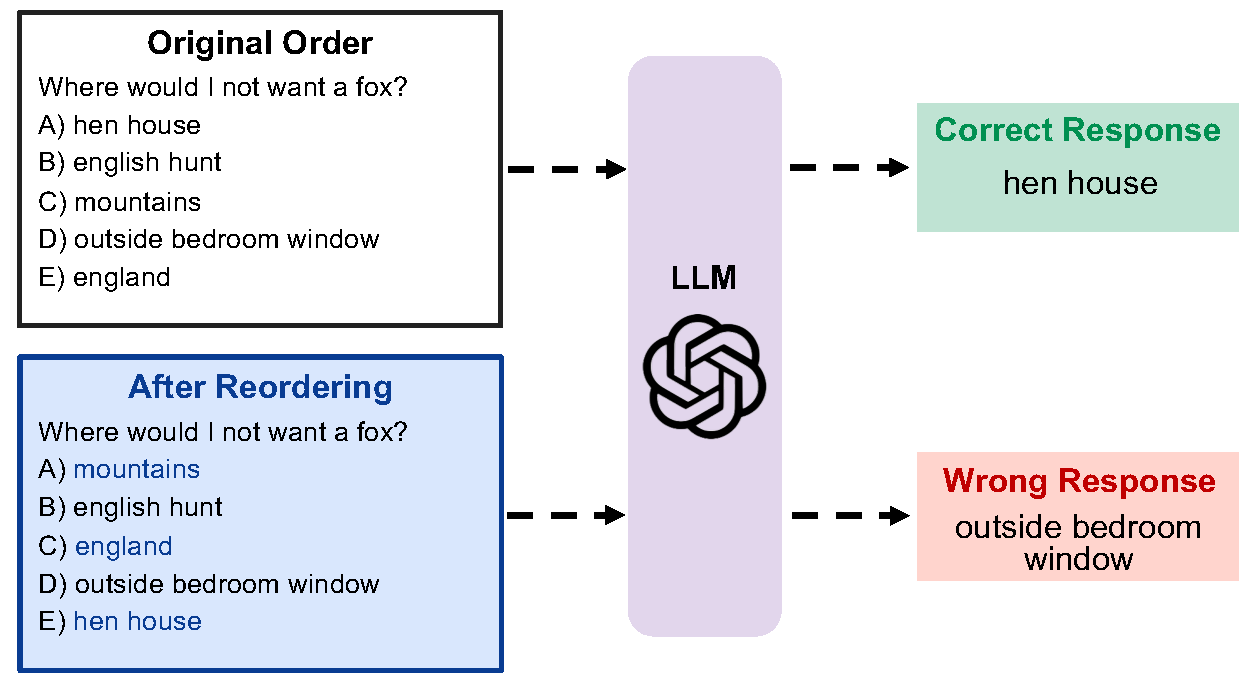
\includegraphics[width=0.7\columnwidth]{submissions/Estevam2024/figures/overview-mcq.pdf}
    \caption{{GPT-4 sensitivity to reordering options:} Upon changing the order of choices, GPT-4 changes its prediction from ``hen house'' to ``outside of bedroom window'' (the example is from the CSQA dataset).}
    \label{fig:over}
     % \minipostspace
\end{figure}

To address the first question, \cite{pezeshkpour2024large} conducted experiments using GPT-4, InstructGPT (text-davinci-003), and Llama-2-13b (chat version) across five multiple-choice question benchmarks. A surprisingly high sensitivity gap of up to 85\% in the zero-shot setting (see Table ~\ref{tab:attack-zero}) was found. Furthermore, in the few-shot setting, introducing demonstrations to the prompt led only to marginal gains in robustness, if any improvement was observed.

\begin{table*}[th!]
\small
\centering
\begin{tabular}{lrrrrrrrrr}
\toprule 
\multirow{2}{*}{\bf Tasks} & \multicolumn{3}{c}{\bf GPT-4}&  \multicolumn{3}{c}{\bf InstructGPT}&  \multicolumn{3}{c}{\bf Llama-2-13b}\\
\cmidrule(lr){2-4}
\cmidrule(lr){5-7}
\cmidrule(lr){8-10}
&Vanila&Min&Max&Vanila&Min&Max&Vanila&Min&Max\\
\midrule
CSQA &84.3&\color{cadmiumred}{-12.6}&\color{cadmiumgreen}{+10.3}&72.3&\color{cadmiumred}{-24.0}&\color{cadmiumgreen}{+19.1}&62.2&\color{cadmiumred}{-28.9}&\color{cadmiumgreen}{+25.5}\\
Logical Deduction&92.3&\color{cadmiumred}{-8.1}&\color{cadmiumgreen}{+5.0}&64.0&\color{cadmiumred}{-39.4}&\color{cadmiumgreen}{+34.7}&53.0&\color{cadmiumred}{-30.7}&\color{cadmiumgreen}{+34.7}\\
Abstract Algebra &57.0&\color{cadmiumred}{-30.0}&\color{cadmiumgreen}{+23.0}&33.0&\color{cadmiumred}{-31.0}&\color{cadmiumgreen}{+39.0}&32.0&\color{cadmiumred}{-32.0}&\color{cadmiumgreen}{+53.0}\\
High School Chemistry &71.9&\color{cadmiumred}{-23.6}&\color{cadmiumgreen}{+18.2}&44.8&\color{cadmiumred}{-28.5}&\color{cadmiumgreen}{+38.0}&40.6&\color{cadmiumred}{-32.7}&\color{cadmiumgreen}{+45.6}\\
Professional Law &66.1&\color{cadmiumred}{-12.7}&\color{cadmiumgreen}{+12.1}&48.6&\color{cadmiumred}{-24.9}&\color{cadmiumgreen}{+25.7}&43.8&\color{cadmiumred}{-32.8}&\color{cadmiumgreen}{+32.9}\\
\bottomrule
\end{tabular}
\caption{\textbf{Zero-shot order sensitivity}; all three LLMs display a notable level of sensitivity to the order of options across various benchmarks.}
\label{tab:attack-zero}
\end{table*}

\begin{figure*}[th!]
    \centering
    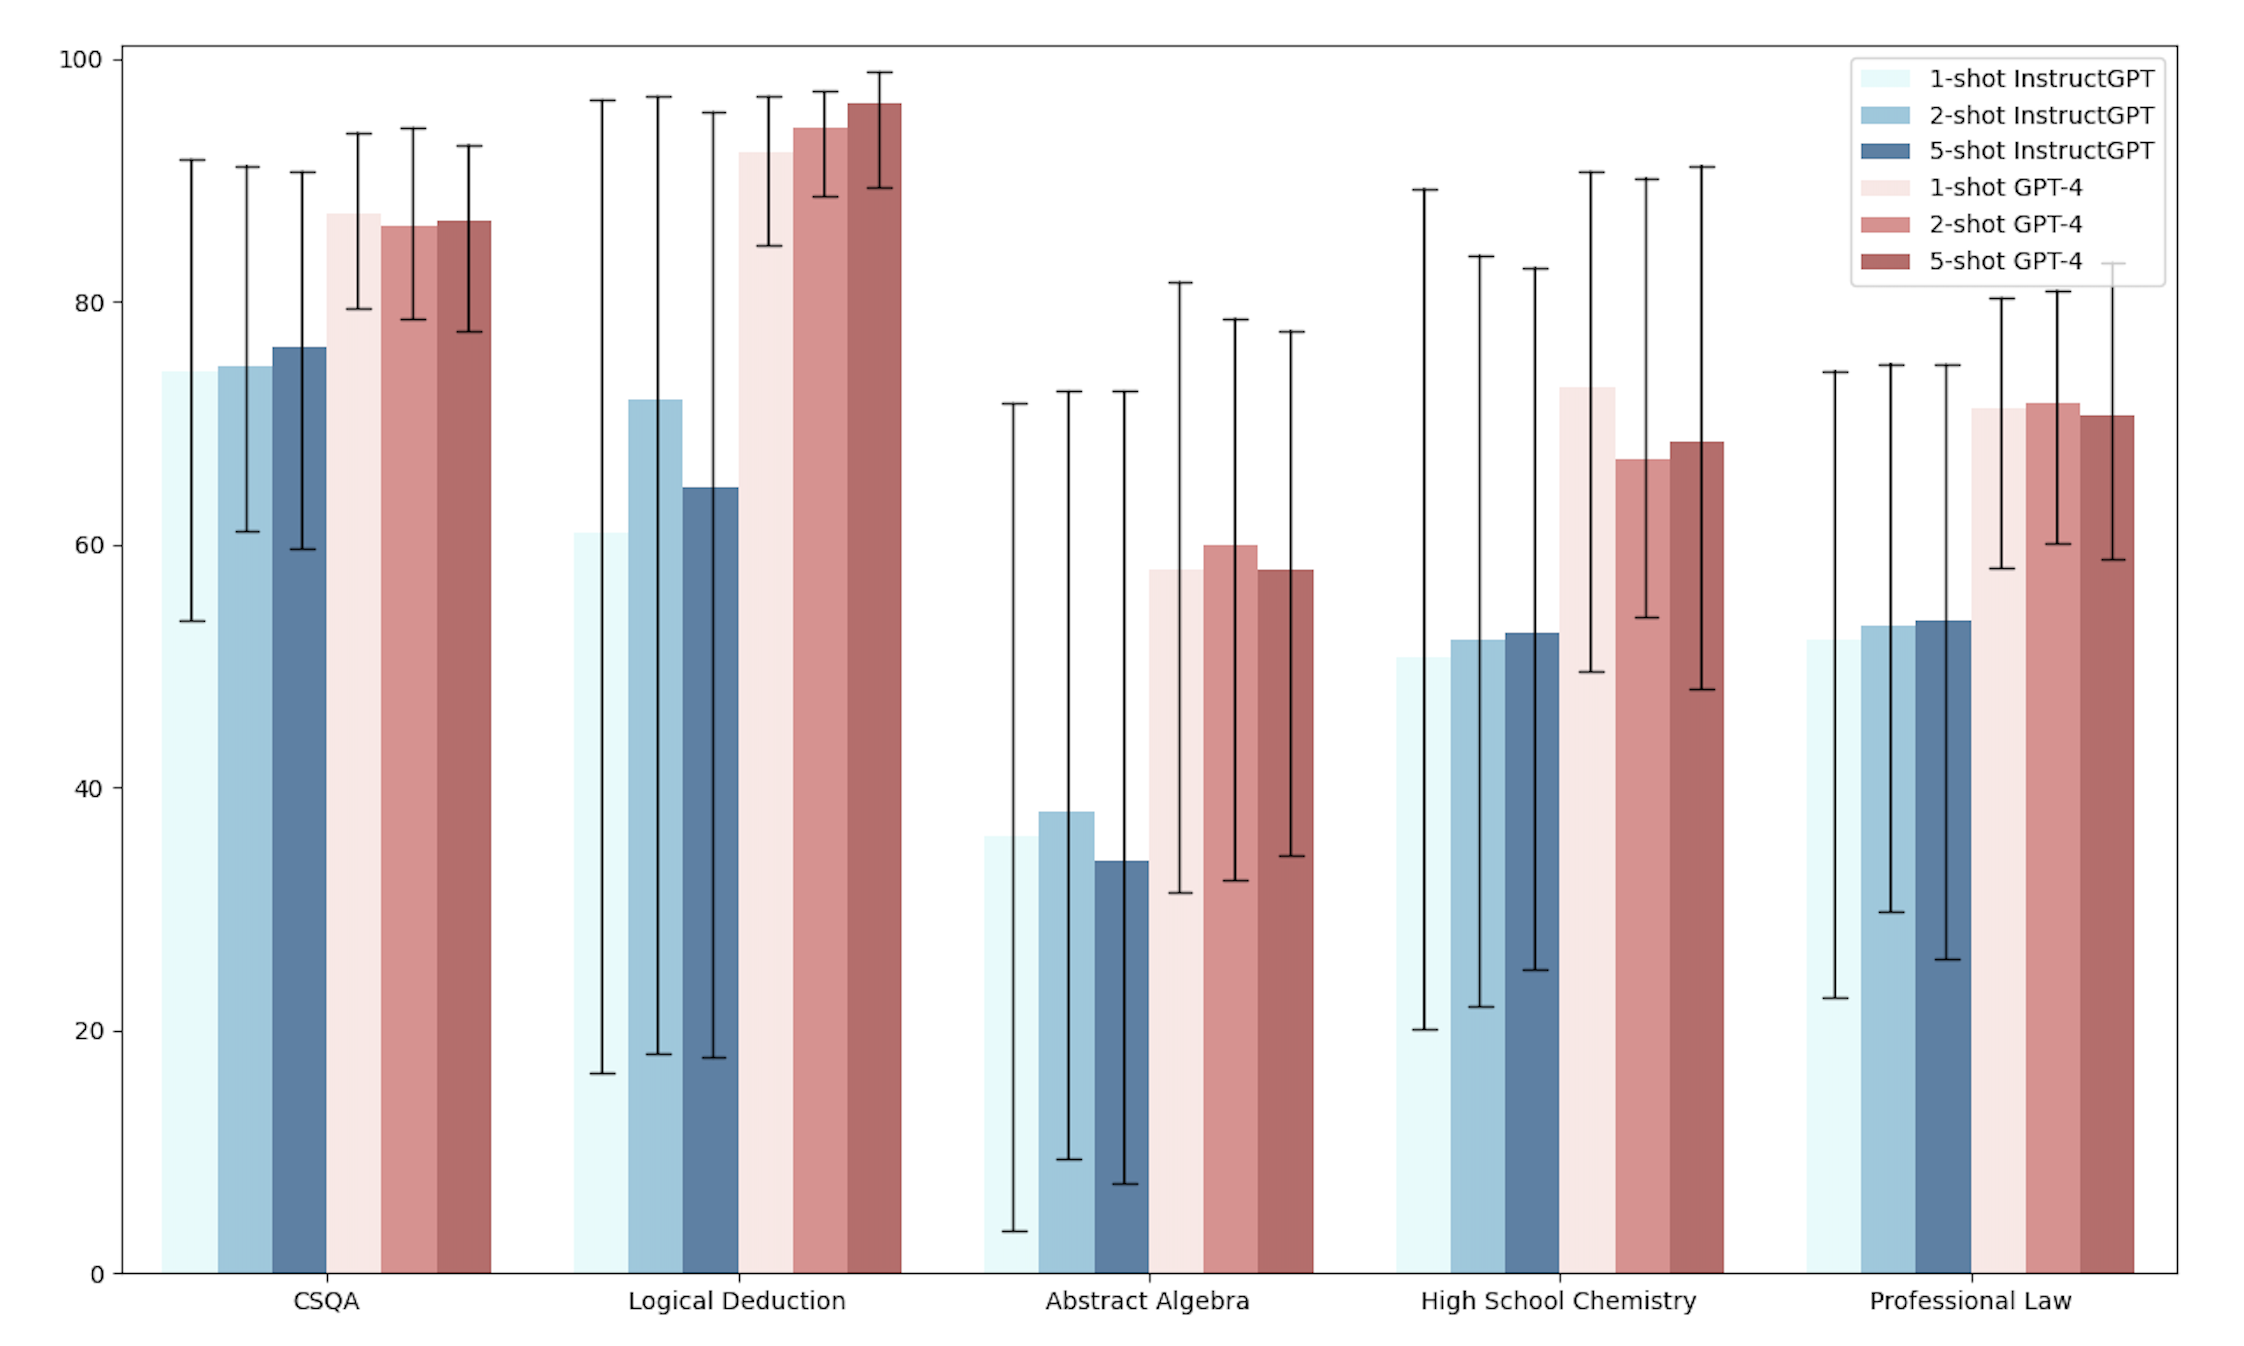
\includegraphics[width=0.5\paperwidth]{submissions/Estevam2024/figures/few-shot-order.png}
    \caption{\textbf{Order sensitivity in the few-shot setting:} The error bars represent the range of minimum and maximum accuracy achievable in each task through oracle reordering. Our observations are as follows: (1) The sensitivity gap consistently remains substantial in the few-shot setting. (2) As performances improve, the sensitivity gap shrinks. (3) Adding more demonstrations does not necessarily results in a reduction of the gap.}
    \label{fig:few-sens}
\end{figure*}

Regarding the second question, it is hypothesized that this sensitivity arises from positional bias, where LLMs display a preference for certain answer placements when uncertain. To investigate, \cite{pezeshkpour2024large} analyzed instances where the models’ predictions shifted upon reordering answer options. Additionally, was also found that increasing the number of options, while keeping the top possible answers, only gradually affected performance, suggesting that positional bias rather than option count plays a larger role in LLM sensitivity (see Figure ~\ref{fig:few-sens}). 

Another interesting finding from \cite{pezeshkpour2024large} is that, instead of using the original order of the multiple-choice options, one can adopt a "system 2" approach and reason before output the first answer generated by the LLM. In this sense, before deciding on the final answer for the question, the same question can be posed to the LLM multiple times (five times in the referenced study), each time with a randomly shuffled set of choices. Afterward, the answers are aggregated through a reasoning mechanism (in the paper, a very simple majority voting reasoning was employed). This approach has been shown to improve the LLM's overall performance.  






%todo
% \subsubsection{Reliable Decision Making w/ RAG}
\subsubsection{Transparency and Accountability in Downstream Applications}
\label{sec:rag_accountable}
To study the implications of trust and accountability of RAG pipelines in downstream applications, \cite{mishra2023characterizing} considers the task of generating natural language explanations of knowledge-intensive task (KIT) decisions such as multiple-choice question answering. Given the setting for generating corroborating and refutation complete rationales for KIT model decisions, the suitability of retrieval-augmented rationale generation using LLMs is explored. The prompt to LLMs is enriched with relevant knowledge from external sources to condition the rationale generation on facts. Three human subject studies were conducted to evaluate the effectiveness of such rationales in communicating KIT model decisions. 

More specifically, two studies were conducted, via crowdsourcing, to evaluate the preferability and acceptability of such rationales to crowd-workers. In another study involving experts --- motivated by existing literature on trust in explainable AI~\cite{hoffman2018metrics, stites2021sage} --- the implications of faithfully rationalizing KIT model decisions irrespective of their correctness was explored.
The crowd-sourced studies demonstrate that, more often than not, crowd workers prefer LLM-generated
rationales to crowdsourced rationales in existing datasets, citing their factuality, sufficiency, and convincing refutation. 
Follow-up fine-grained analysis 
reveals that LLM-generated rationales
still have significant room for improvement along
dimensions such as \emph{insightfulness} (\ie providing new information), \emph{redundancy} (\ie avoiding repetitive text), and \emph{generalizability} (\ie domain invariance.)
The expert-sourced study confirms that faithful rationalization of incorrect model predictions 
degrades humans' trust in the generated rationales. 
The work further explores the utility of instrumenting mechanisms
to intervene in the incorrect predictions via a review-then-rationalize pipeline instead of faithfully rationalizing and find that even simple strategies may help intervene up to $71\%$ of the incorrect predictions.

\begin{figure} 
\vspace{-10pt}
    \centering
    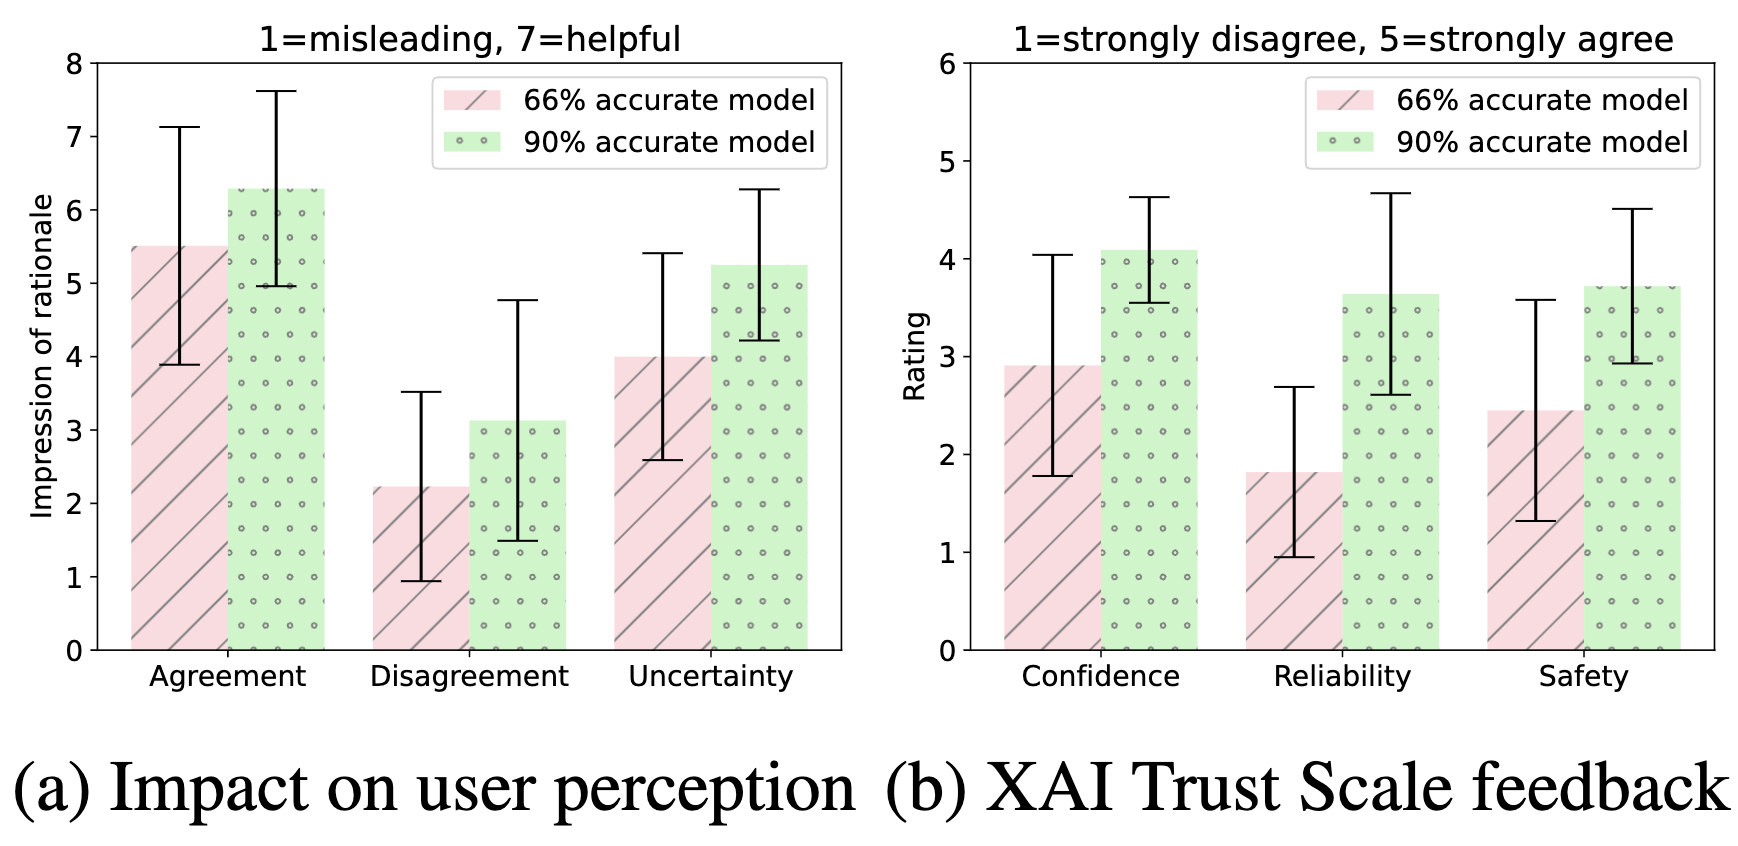
\includegraphics[width=0.6\linewidth]{submissions/Estevam2024/figures/xai-trust.png}
 
  \caption{(a) Irrespective of agreement or disagreement with the KIT model prediction, participants indicated a more negative impression about the rationalization of the lower confidence model prediction. (b) Participant feedback on the trust scale indicates lower confidence for lower accuracy model rationalization.}
  \label{fig:xai_rationale} 

\end{figure}

Figure~\ref{fig:xai_rationale}a \cite{mishra2023characterizing} summarizes the participants' impression of a rationale immediately after viewing the model prediction. When the participants disagreed with the model prediction, they exhibited a stronger negative impression about the rationales for the $66\%$ accuracy condition compared to the $90\%$ accuracy condition. Even when participants agreed with the model prediction, their impression of the rationales remained more negative. The intuition is that the higher disagreement with the model coupled with observing the faithful rationalization of the incorrect prediction negatively impacted participants' perception of the reliability of the rationales. These observations are confirmed by analyzing the results of the follow-up survey (see Figure~\ref{fig:xai_rationale}b.)  Unsurprisingly, participants for the $66\%$ accuracy condition rated their confidence in the generated rationales and the reliability of the rationalizer significantly lower compared to the $90\%$ accuracy condition.




\section{Towards System 2 RAG in the wild}

% \subsubsection{Monolithic models to compound AI systems}

Towards productizing generative AI, there has been a shift from monolithic models to compound AI systems~\cite{kandogan2024blueprint} that incorporate various components other than LLMs for data retrieval, coordination, and utilizing proprietary models and services. Examples of such systems include Hiring Assistant by LinkedIn~\cite{linkedin-assistant}, AI-BI Genie by Databricks~\cite{databricks-aibi}, Agentforce by Salesforce~\cite{salesforce-agentforce}, and Magentic-One by Microsoft~\cite{microsoft-magentic}, among others. These systems are designed to ensure performance for complex tasks, adaptability to heterogeneous data and use cases, and a higher degree of trust in the production setting.

\stitle{Motivating example.}
Consider LinkedIn and Indeed, two global job-matching and hiring platforms in the HR domain. These companies are employing RAG-based workflows for a multitude of tasks in HR, such as matching, recruitment, and career guidance, among others~\cite{indeed-ai-blog, linkedin-ai-blog}. 
Given the task of matching job seekers with job postings, a popular use-case of generative AI is communicating meaningful explanations to job seekers about their relevance to the job. To support such a use-case, enterprises use RAG to infuse domain-specific relevant information, which guides the generation of explanations using LLMs~\cite{indeed-ai-blog}. Identifying the relevant information to be provided to the LLM in such a domain-specific context can be challenging due to the heterogeneity and scale of the data. Moreover, within such a production-oriented setting, enterprises have to remain cognizant of real-world constraints such as cost, latency, accuracy, and trustworthiness.


% \subsubsection{Data Heterogeneity}

\subsection{Data Heterogeneity in the Wild}
 Within an enterprise setting, different teams in an organization manage project-specific sources of data, collected and often transformed through various workflows over time. Such an observation is derived from the authors' experience working with enterprise data in the human resources (HR) domain at \company. 
For example, going back to the example of explaining job seeker and job posting match, a team tasked with such work will be interested in unstructured resumes and job descriptions, structured data extracted from the text and their representations, and HR domain-specific knowledge, \ie, relationships among different concepts such as jobs and benefits. Another team working on assisting job-seekers with search (\eg role and company) will be more interested in rather job market trends, company-specific information and search logs, among others. 

\begin{figure}[!htb] 
  \centering
  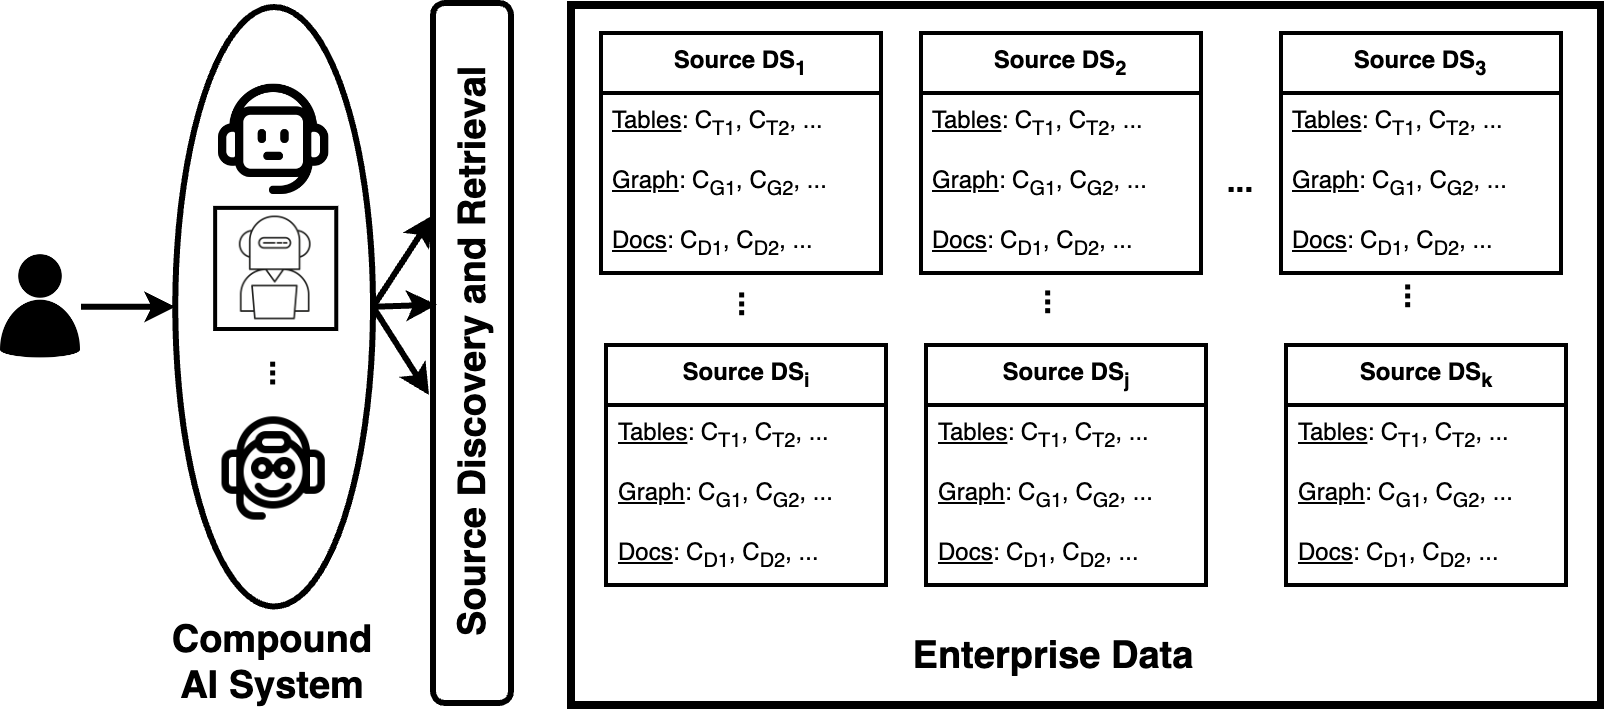
\includegraphics[width=0.65\linewidth]{submissions/Estevam2024/figures/mmd-lake.drawio.png}
  \caption{Conceptual data model for RAG in the wild.}
  \label{fig:cas_enterprise} 
\end{figure}

We introduce the data model for such a setting in Figure~\ref{fig:cas_enterprise}: \emph{compound AI systems} operating over such enterprise data~\cite{feng2024cmdbench}. The data model is multi-granular and multi-modal. Each team-specific data source $DS_i$ represents a collection of sources ($S_m \in DS_i$) corresponding to different modalities ($m$)  --- such as multiple tables and documents --- created by specific teams. While enterprises may contain data corresponding to other modalities such as audio, video, and image, we limit our scope to documents ($m=D$), tables ($m=T$), and graphs ($m=G$) in this case. Each data source is organized in a hierarchical manner --- at the coarse-grained level data is organized in data sources $DS_i$. Within each data source, data is organized in various collections $C_m$ depending on the modality. Within each collection, data can be stored and managed by different systems ($C_{mi}$) depending on the downstream application such as data warehouse, data lake, and lakehouse systems~\cite{DBLP:journals/bdcc/NambiarM22,armbrust2021lakehouse}. Therefore, the assumption of traditional RAG where these data sources or collections or databases are known beforehand, breaks down in such a setting. Rather a multi-step approach to data discovery (closer to System 2) is required to identify the relevant coarse- and fine-grained data given a user query.

%\subsection{System considerations}
%\begin{figure}[!htb] 
%  %\vspace{-10pt}
%  \centering
%  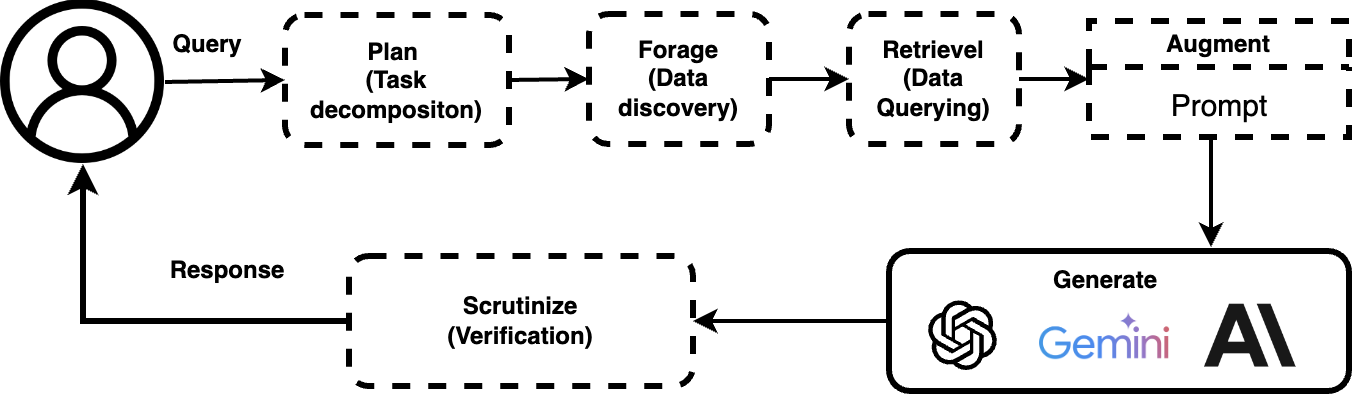
\includegraphics[width=0.8\linewidth]{submissions/Estevam2024/figures/cas-rag.drawio.png}
%  \caption{``System 2'' approach to RAG on enterprise infrastructure through agentic $workflows}
%  \label{fig:sys-rag} 
%  %\vspace{-15pt}
% \end{figure}

\subsection{Rethinking RAG}
To this end, a major consideration in moving a RAG pipeline from System 1 to System 2 thinking involves shifting toward deliberate analytics and explicit reasoning.
This transition means that decisions—such as when and where to retrieve information, how much data to retrieve, and how to integrate retrieved information into the generated response—should be made through rigorous reasoning. This reasoning should carefully assess the unique characteristics of the task, data, tools, and available models to ensure outcomes that are both optimal and context-aware. Note that recently released LLM such as \emph{o1}\footnote{https://openai.com/o1/} instruments slow thinking by executing some type of reasoning mechanism before generating the final answer. Even though there has been discussions within certain research circles, which mentions the possibility of having chain of thought and self-reflection empowering \emph{o1} models before they generate an answer, it is important to state that no official documentation confirms the use of such techniques in the \emph{o1} models) ---- One consequence of this new reasoning capabilities of these models is the additional time spent thinking, that makes it more effective for complex reasoning tasks, particularly in science and mathematics. 
However, the additional step leads to higher latency during inference, which may vary depending on the task. In addition to that, \emph{o1} is similar to the earlier monolithic LLMs where the parametric knowledge remains abstract, thereby lacking transparency and controllability as no affordances are provided to the users to interact with the decision-making process.

 
Given a knowledge-intensive task that requires complex reasoning and planning, a systematic approach is necessitated to ensure transparency of the workflow, integrate user guidance at various steps, and enable optimization under real-world constraints such as cost, latency, and accuracy. As illustrated in Figure~\ref{fig:sys-rag2}, at the core of the System 2 RAG pipeline lies a planner, which functions as a reasoning module. 
This planner is grounded in specific tasks and budgets (\eg time, cost, quality) and operates by foraging and analyzing the properties of data and agents within the registries. Moreover, retrieval is expanded to not only extracting information from documents but also other formats of raw data and data management systems as outlined in Figure~\ref{fig:cas_enterprise}. Adaptation of retrieval to large-scale heterogenous data necessitates reconciliation and reranking of retrieved information. With the presence of heterogeneous information, the augmented generation requires further scrutinization through fact-checking and verification,

% \section{Towards System 2 RAG \todo{revisit section name}}
\section{Design components}
\label{sec:sys2}
%todo 



To achieve effective System 2 RAG pipelines, it is essential to address challenges in both data and model aspects. System 2 decision-making relies on an organized, contextually rich data pool for informed outcomes, making efficient identification and organization of relevant information critical. Data enhancements, such as data discovery agents, play a key role by locating, structuring, and tagging pertinent data to create a streamlined and accessible knowledge base. Similarly, selecting and configuring models for each task is crucial. Choosing the right model, tuning it to align with user expectations, and ensuring seamless integration with the data pipeline all contribute to achieving optimal performance. 
In this section, we provide a high-level overview of our work in tackling these data and model challenges in developing a System 2 RAG pipeline.
\subsection{Data-level enhancements}


\subsubsection{Data Discovery}
As an initial effort to understand the potential impact in the data discovery task, we adapted existing datasets and benchmarks in open-domain --- from question answering and complex reasoning tasks to natural language querying over structured data --- to evaluate coarse- and fine-grained data discovery and task execution performance. Our experiments reveal the impact of data retriever design on downstream task 
  performance --- $46\%$ drop in task accuracy on average ---
  across various modalities, data sources, and task difficulty. The results indicate the need to develop optimization strategies to identify appropriate LLM agents and retrievers for efficient execution of CASs over enterprise data. This need is well-aligned with the System 2 type of thinking, in which before performing the retrieval, there is a need for reasoning on what data is available and how it should be retrieved. After such a reasoning step, the retrieval (and the RAG results in general) have the potential to improve.

 

\begin{figure}[!htb]
    \centering
    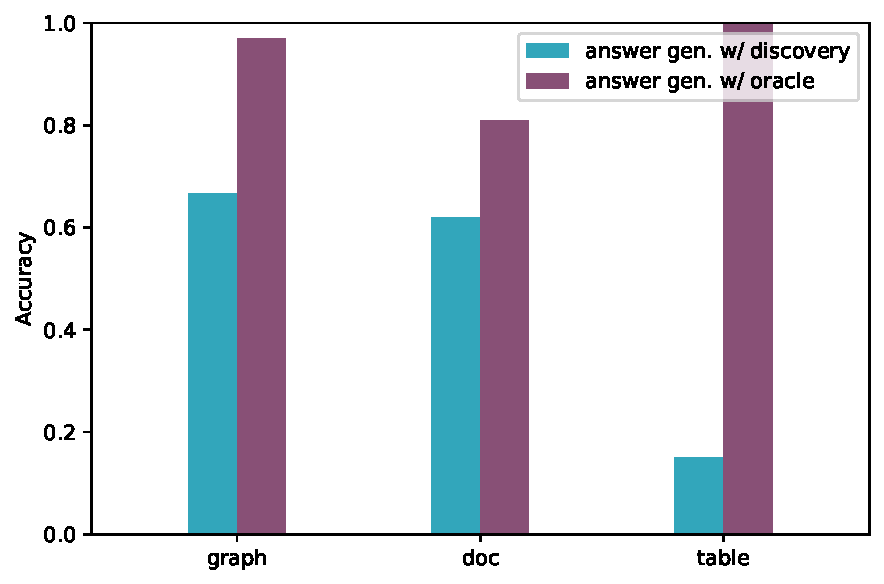
\includegraphics[width=0.5\linewidth]{submissions/Estevam2024/figures/answer_gen.pdf}
    \caption{Task execution performance degrades due to poor data discovery despite the purported proficiency of LLMs. }
    \label{fig:answer_gen}
    \vspace{-10pt}
\end{figure}

When we explored the impact of data discovery performance on the accuracy of downstream task execution. Figure~\ref{fig:answer_gen} captures the task execution accuracy for two scenarios: oracle and discovery. Oracle is the case where the ground truth discoverable element is provided to the LLM (\eg GPT-3.5 turbo) to provide the final answer to a question. Discovery captures the scenario where elements retrieved by the best-performing document, sub-graph, and table discovery models are provided to the LLM. We observe a significant drop in performance from \emph{oracle} to the \emph{discovery} scenario,  showcasing a $46\%$ decrease in accuracy.

\subsubsection{Less is More for Evaluation}


Evaluating text generation is crucial for creating high-quality systems. However, aligning automatic evaluation metrics with human judgment remains challenging~\cite{bhandari-etal-2020-evaluating,fabbri2021summeval}. While LLMs demonst
rate promising correlations with human evaluations, they encounter issues like high costs and the Lost-in-the-Middle problem~\cite{liu2023lost}, where key information in the middle of lengthy documents is frequently overlooked in summary evaluations.

To tackle these challenges, \cite{wu2024less} introduced a straightforward yet effective approach known as \textit{Extract-then-Evaluate}. At run-time, this method begins by extracting significant sentences from a lengthy source document and concatenating them until the extracted text reaches a predefined length. Subsequently, it assesses the quality of the summary based on this extracted content using LLMs. Figure ~\ref{fig:less_is_more} shows the overview of our approach. Notice that \emph{Extract-then-Evaluate} brings a System 2 type of thinking. The evaluation requires the analysis of the original document and the identification of the key elements. Only after reasoning and identifying such key elements is the evaluation of the quality of the summary performed.

\begin{figure}[!t]
  \centering
  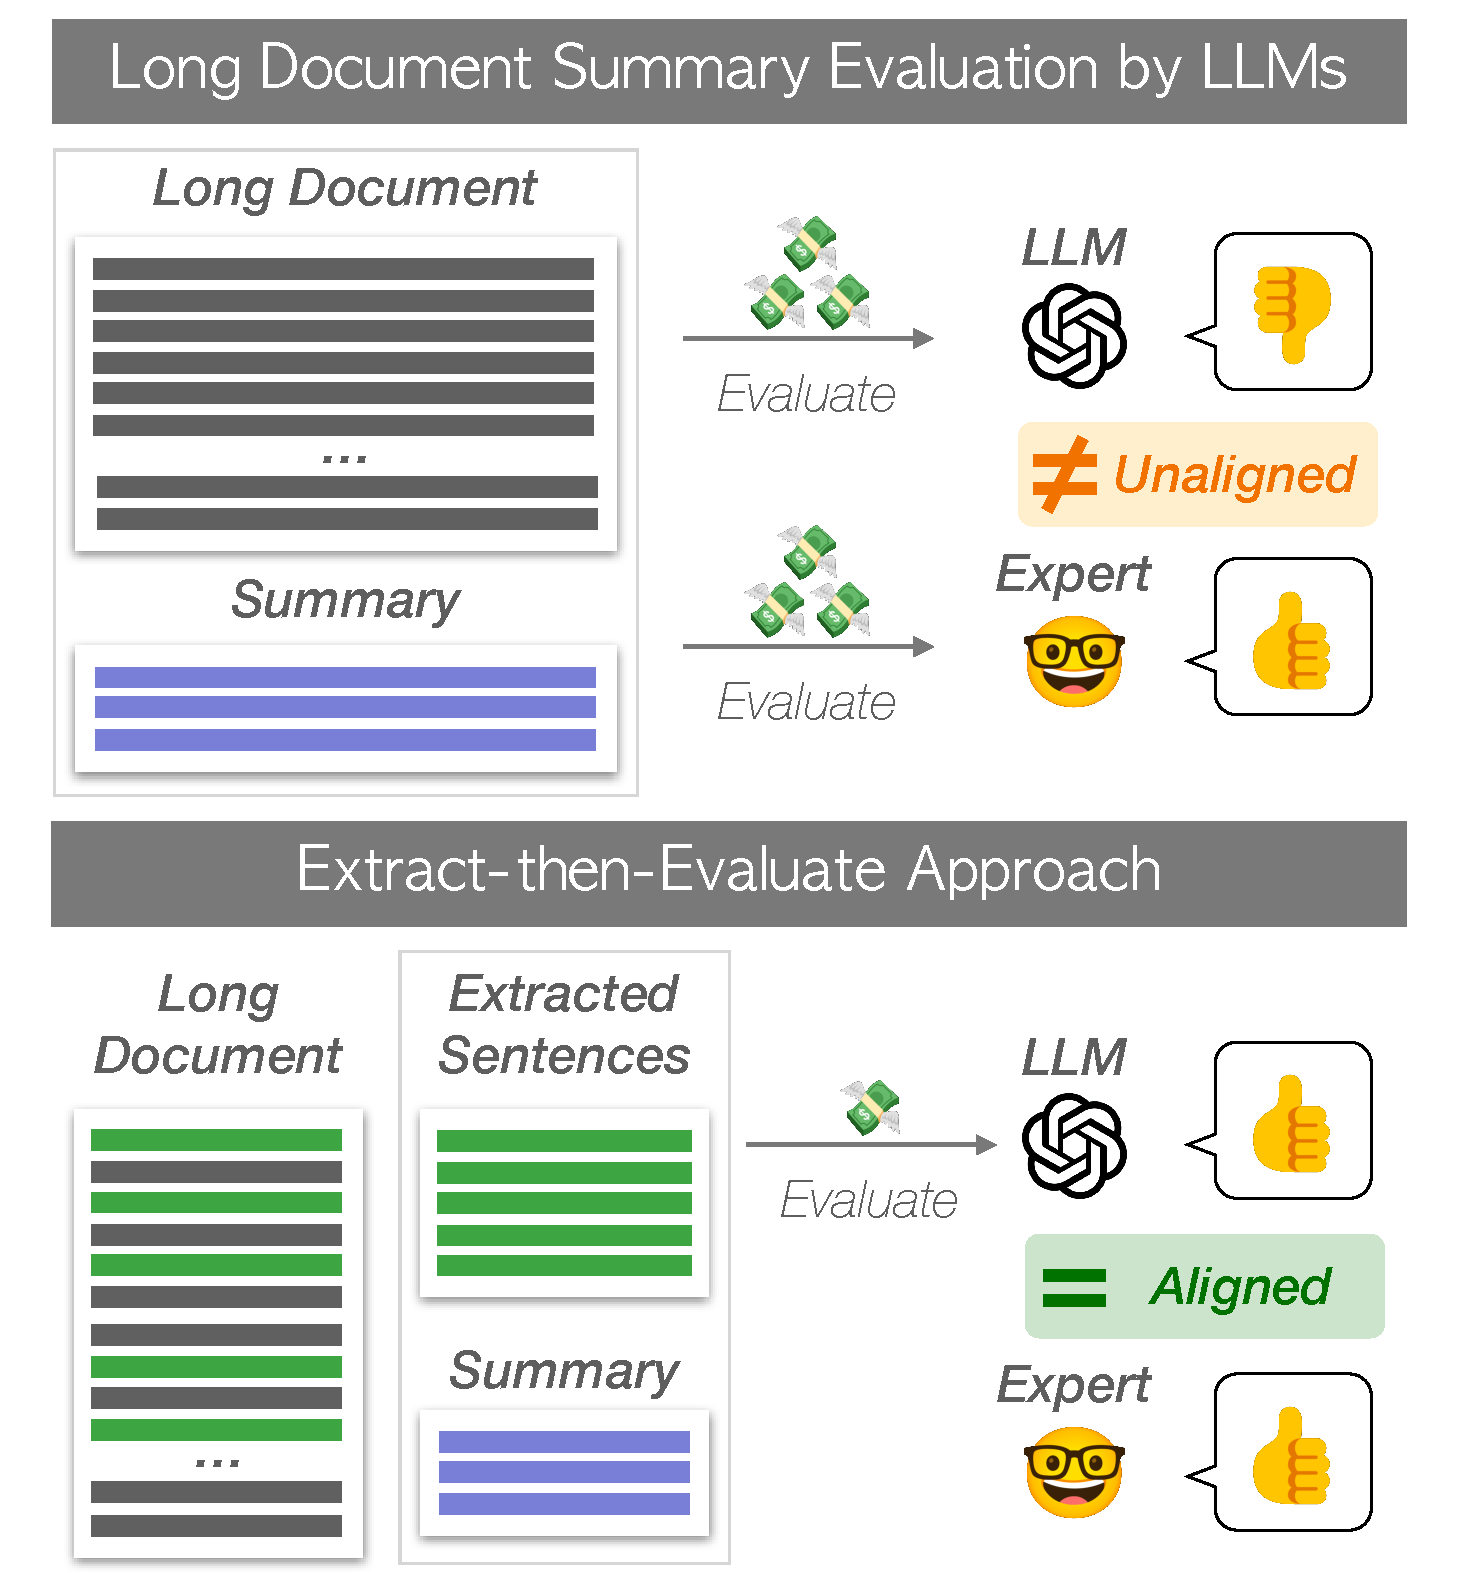
\includegraphics[width=0.5\linewidth]{submissions/Estevam2024/figures/less_is_more.pdf}
  \caption{Overview of the long document summary evaluation task by LLMs. Evaluating long document summaries by LLMs is expensive and shows limited alignment with human evaluations. This study demonstrates that extracting important sentences for evaluation in advance not only reduces evaluation costs but also exhibits better alignment with human evaluations.}
  \label{fig:less_is_more}
\end{figure}

The experiments explore various sentence extraction techniques, encompassing both matching-based and model-based methods, such as LEAD, ROUGE, BERTScore, and NLI. Their performance is evaluated across multiple datasets, including arXiv, GovReport, PubMed, and SQuALITY~\cite{koh-etal-2022-far,krishna-etal-2023-longeval}. The main results are shown in Table~\ref{tab:less_is_more_main_result}. In the experiments, LLMs demonstrated a notable enhancement in correlation with human judgment when compared to non-LLM baselines. However, this improvement came with increased evaluation costs due to the full document prompt length. Extracting key information before evaluation not only reduced costs but also improved performance, attributed to the Lost-in-the-middle problem, where LLMs struggle with critical information in lengthy documents. This trend showed that LLMs perform better with shorter, more informative documents. Lastly, even within a limited budget, the approach delivered comparable performance to top configurations, achieving similar results to the best extraction method while cutting evaluation costs in half.

Based on these observations, it is possible to conclude that effective data pre-processing can reduce costs while allowing the model to concentrate on key information, ultimately enhancing performance.

\begin{table*}[th!]
    \centering
    \small
    \resizebox{\textwidth}{!}{
    \begin{tabular}{lcccccccccccccccccc}
        \toprule
        & \multicolumn{6}{c}{\textbf{Consistency}} & \multicolumn{6}{c}{\textbf{Relevance}} & \multicolumn{6}{c}{\textbf{Faithfulness}}\\
        & \multicolumn{3}{c}{\textbf{arXiv}} & \multicolumn{3}{c}{\textbf{GovReport}} & \multicolumn{3}{c}{\textbf{arXiv}} & \multicolumn{3}{c}{\textbf{GovReport}} & \multicolumn{3}{c}{\textbf{PubMed}} & \multicolumn{3}{c}{\textbf{SQuALITY}} \\
        \cmidrule(lr){2-4} \cmidrule(lr){5-7} \cmidrule(lr){8-10} \cmidrule(lr){11-13} \cmidrule(lr){14-16} \cmidrule(lr){17-19} 
        \textbf{Methods} & $r$ & $\rho$ & $\pounds$ & $r$ & $\rho$ & $\pounds$ & $r$ & $\rho$ & $\pounds$ & $r$ & $\rho$ & $\pounds$ & $r$ & $\rho$ & $\pounds$ & $r$ & $\rho$ & $\pounds$ \\\midrule
        \multicolumn{19}{c}{\textit{Reference-based metrics}}\\
        \midrule
        ROUGE-1 & -0.08 & -0.13 & - & -0.12 & -0.11 & - & 0.29 & 0.25 & - & 0.53 & 0.52 & - & 0.32 & 0.30 & - & -0.33 & -0.13 & -\\
        BERTScore & -0.09 & -0.10 & - & 0.00 & -0.04 & - & 0.22 & 0.18 & - & 0.38 & 0.38 & - & 0.49 & 0.49 & - & -0.12 & 0.02 & -\\
        BARTScore & 0.32 & 0.36 & - & 0.51 & 0.48 & - & 0.00 & 0.03 & - & 0.18 & 0.24 & - & 0.49 & 0.47 & - & -0.06 & -0.17 & -\\
        \midrule
        \multicolumn{19}{c}{\textit{Reference-free metrics}}\\
        \midrule
        FactCC & 0.22 & 0.19 & - & 0.28 & 0.27 & - & 0.13 & 0.13 & - & 0.05 & 0.04 & -  & -0.09 & -0.14 & - & 0.13 & 0.14 & -  \\
        SummaC & 0.32 & 0.32 & - & 0.39 & 0.38 & - & 0.09 & 0.08 & - & 0.05 & 0.04 & - & 0.51 & 0.55 & - & 0.18 & 0.24 & -\\
        \midrule
        \multicolumn{19}{c}{\textit{Reference-free metrics with LLM} (ours)}\\
        \midrule
        Full document & 0.61 & 0.46 & \$0.15 & 0.33 & 0.34 & \$0.10 & 0.58 & 0.52 & \$0.15 & 0.12 & 0.11 & \$0.10 & 0.64 & 0.70 & \$0.11 & 0.51 & 0.38 & \$0.14 \\
        Best extraction & 0.71 & 0.50 & \$0.05 & 0.62 & 0.60 & \$0.09 & 0.63 & 0.58 & \$0.07 & 0.36 & 0.40 & \$0.07 & 0.76 & 0.80 & \$0.07 & 0.85 & 0.81 & \$0.04\\
        Pareto efficient & 0.71 & 0.50 & \$0.05 & 0.60 & 0.61 & \$0.05 & 0.55 & 0.48 & \$0.04 & 0.37 & 0.37 & \$0.05 & 0.75 & 0.75 & \$0.05 & 0.85 & 0.81 & \$0.04\\
        \bottomrule
    \end{tabular}}
    \caption{Results for Pearson correlation ($r$), Spearman correlation ($\rho$), and the average evaluation cost per instance ($\pounds$) indicate that extracting important sentences before evaluation (Best extraction) can yield a higher correlation. Even under a limited budget (Pareto efficient), these results show comparable or even higher correlations compared to the full document setting, with lower costs.}
    \label{tab:less_is_more_main_result}
\end{table*}

\subsection{Model-level enhancements}


Despite ongoing advancements in LLM and RAG models and their continual scaling, there appears to be no clear limit to their growth potential. As a result, integrated systems and workflows—often called compound systems or agentic workflows—are emerging. 
These systems combine LLMs with multiple components, including repeated model calls, retrievers, and external tools, through commercial frameworks like LangChain, LlamaIndex, Auto-GPT, and AgentGPT. Such frameworks empower developers to create agents with unique decision-making capabilities, specialized expertise, and integration with proprietary systems or datasets, as well as build diverse applications ranging from customer service chatbots to advanced decision-support systems. We now highlight several research efforts that showcase compound systems designed to address complex NLP tasks and emphasize that the presence of a System 2 type enhances the performance in such complex tasks.  


\subsubsection{Multi-conditional ranking}

Ranking items based on multiple conditions has wide-ranging applications across various fields. In recommendation systems, for example, once top candidates are shortlisted, re-ranking them according to specific conditions—like genre or category—can greatly enhance the user experience. Similarly, in competitive job markets, this approach is essential for matching resumes to job postings, allowing for prioritization by skills, experience, and other relevant factors.  While there has been considerable advancement in ranking extensive document collections given a query \cite{khattab2020colbert,zhuang2023setwise,qin2023large}, the nuanced task of ranking a smaller set of items based on multiple conditions has not been addressed in prior research.


\begin{figure*}[th!]
    \centering
    \begin{subfigure}[b]{0.24\textwidth}
        \centering
        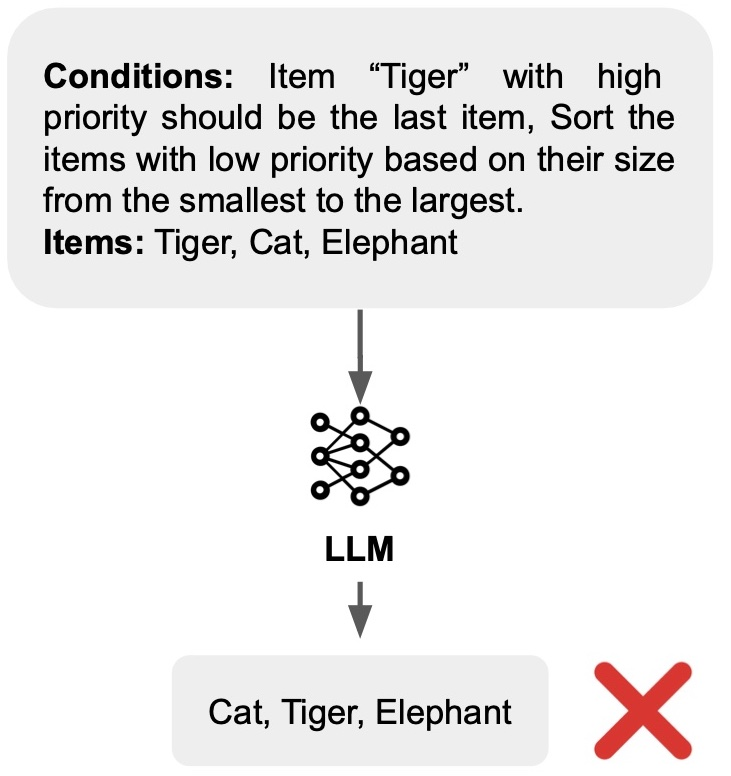
\includegraphics[width=\linewidth]{submissions/Estevam2024/figures/overview-base.jpg}  
        \caption{Base Approach}
    \end{subfigure}%
    ~ 
    \begin{subfigure}[b]{0.65\textwidth}
        \centering
        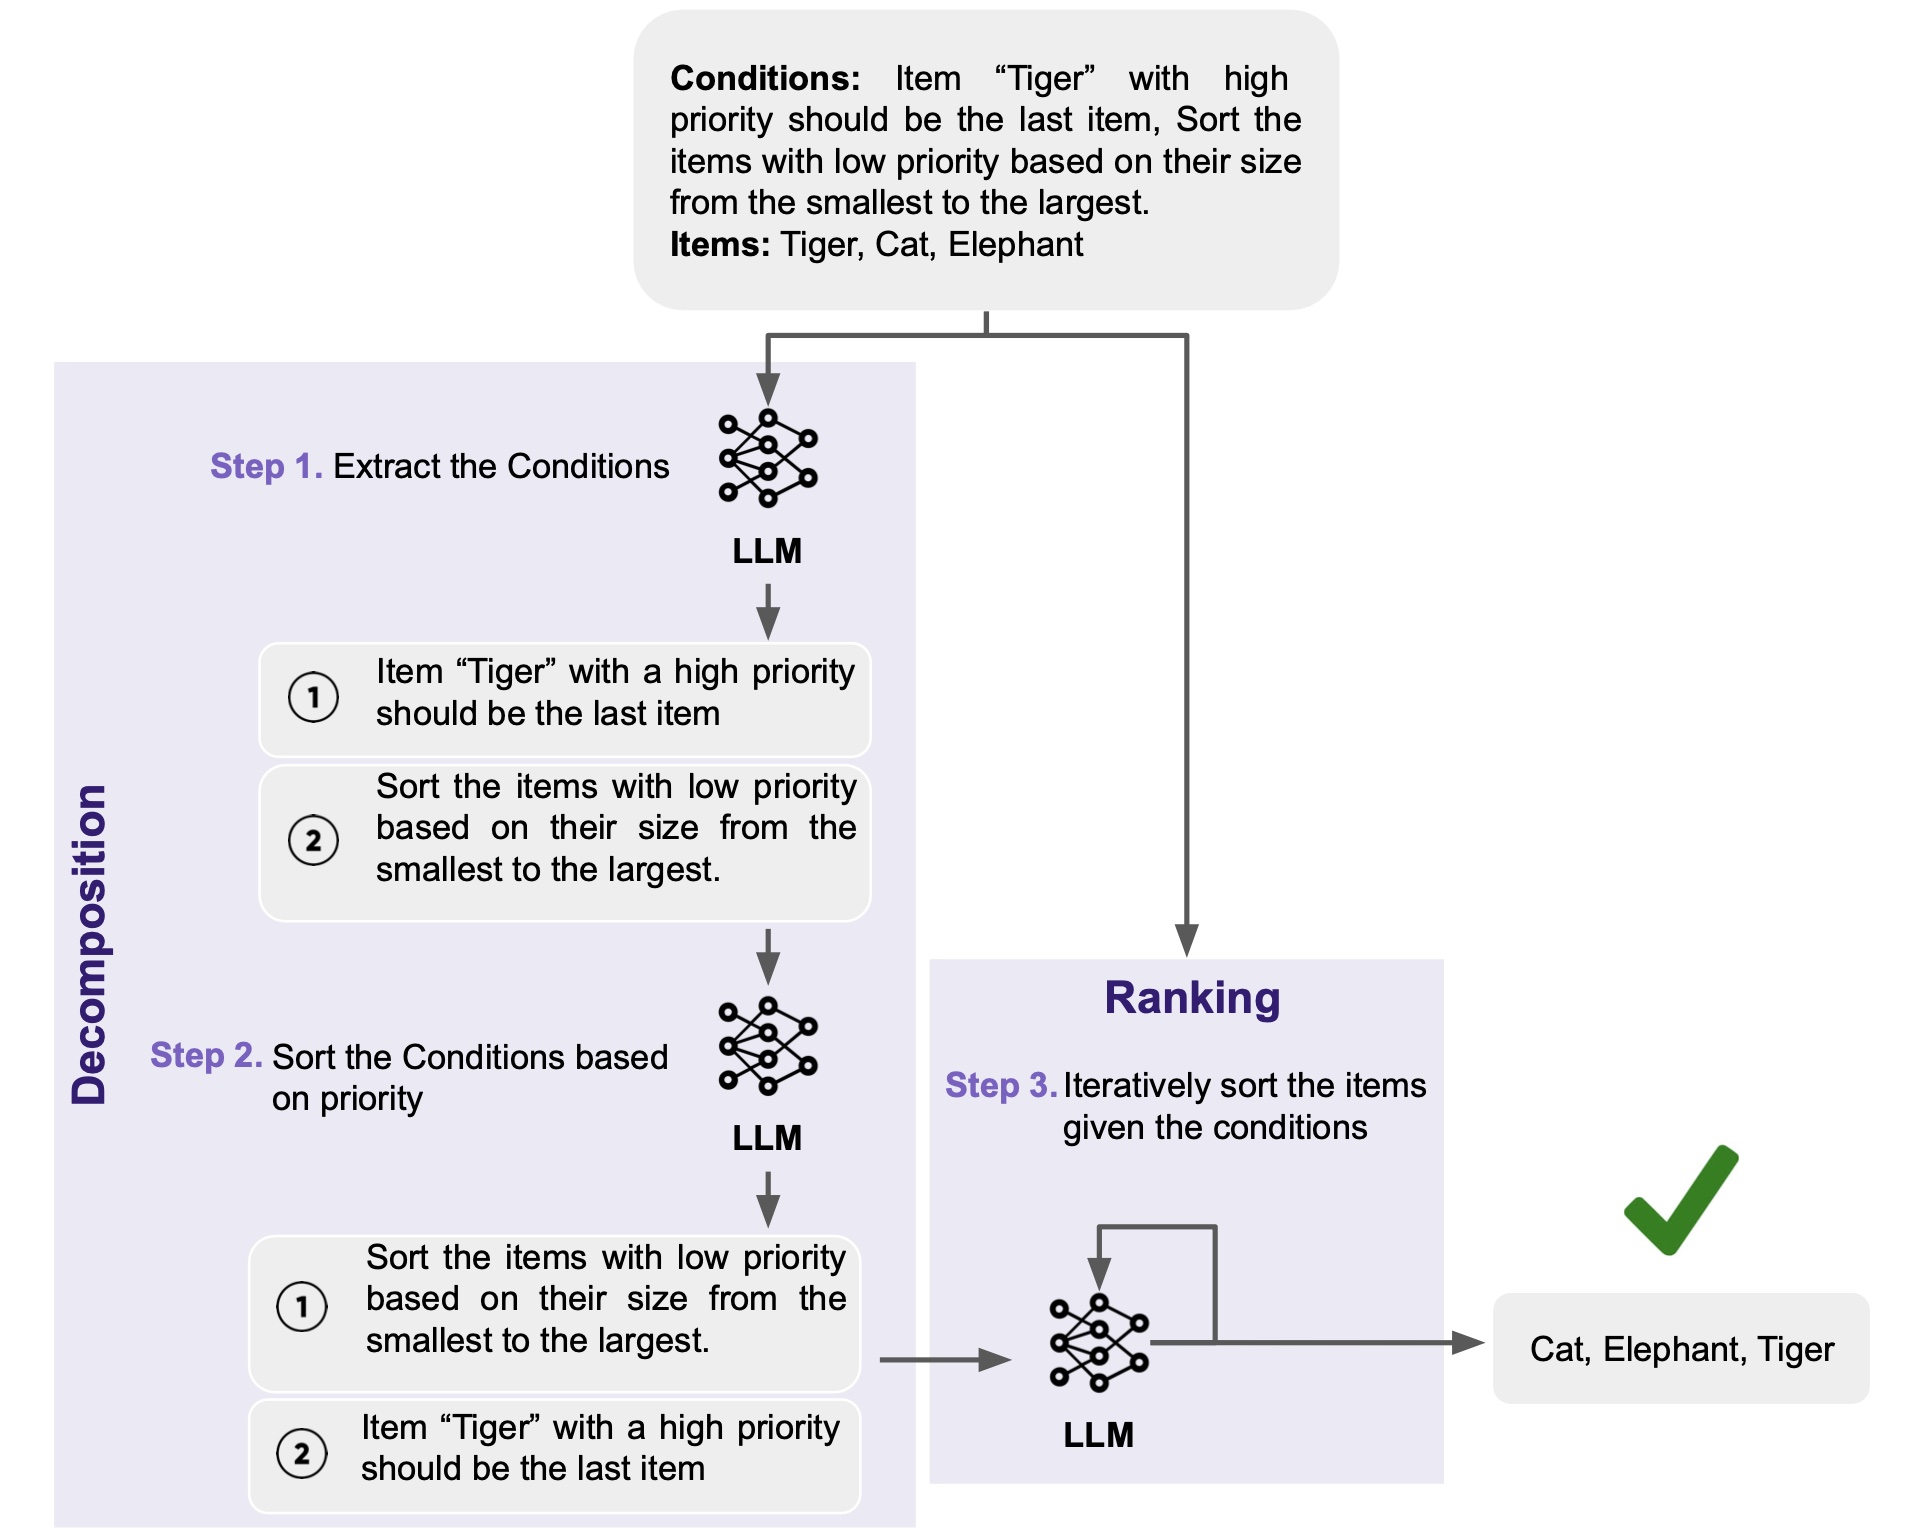
\includegraphics[width=\linewidth]{submissions/Estevam2024/figures/overview-exsir.jpg}
        \caption{EXSIR (Ours)}
    \end{subfigure}  
    \caption{Overview of multi-conditional ranking. Instead of directly prompting LLMs to rank items based on the given conditions, we first extract and sort the conditions based on their priority. Then, we iteratively apply these sorted conditions to the item list.}
    \label{fig:mcr}
\end{figure*}

To address this gap, \cite{pezeshkpour2024multi} defines and investigates the task of multi-conditional ranking (MCR) through the introduction of MCRank, a comprehensive benchmark that encompasses various item types and ranking conditions for evaluating MCR performance. MCRank includes a diverse array of conditions, including positional, locational, temporal, trait-based, and reasoning conditions. Specifically, MCRank was developed by creating a dataset with 18 scenarios varying in item categories, number of conditions (1, 2, or 3), and item set sizes (3, 5, or 7). Each scenario included 200 samples, generated by compiling data and labels for different condition types, featuring randomly ordered item sets with correct rankings. Positional conditions were sourced from Big-Bench's auto-categorization task and Amazon reviews. For scenarios requiring multiple conditions, additional criteria like character counts or positional conditions were added to simulate realistic complexity. This process ensured a robust dataset for evaluating holistic reasoning in scenarios that simulate situations close to real-cases in which users want to rank items based on different conditions defined by their own needs.

Furthermore, we develop EXSIR, a novel decomposed reasoning method that iteratively refines rankings. The process begins with extracting individual conditions from a given string and organizing them into a coherent list. A sorting mechanism then arranges these conditions based on their assigned priorities. Finally, the sorted conditions are applied iteratively to the item list, refining the rankings in each cycle based on the current condition. Figure \ref{fig:mcr} illustrates the workflow of EXSIR along with an example of MCRank.


Initial investigations into existing LLM performance on MCRank show a clear decline in accuracy as both the number of items and conditions increase. Specifically, we observe a sharp drop in ranking accuracy for LLMs like OpenAI o1-mini, GPT-4, ChatGPT (both turbo versions), Llama 3.1-70B, and Mistral (7B) when tasked with three conditions and seven items, with accuracy nearing 0\%.  EXSIR improves ranking accuracy on MCRank by up to 14.4\%, outperforming strong baselines such as Chain-of-Thought (CoT) (see Figure ~\ref{fig:tok-bar}). These results demonstrate how the initial steps towards the System 2 type of thinking (present in the EXSIR approach) allowed to improve the performance of even very strong baselines. 

\begin{figure*}[th!]
    \centering
    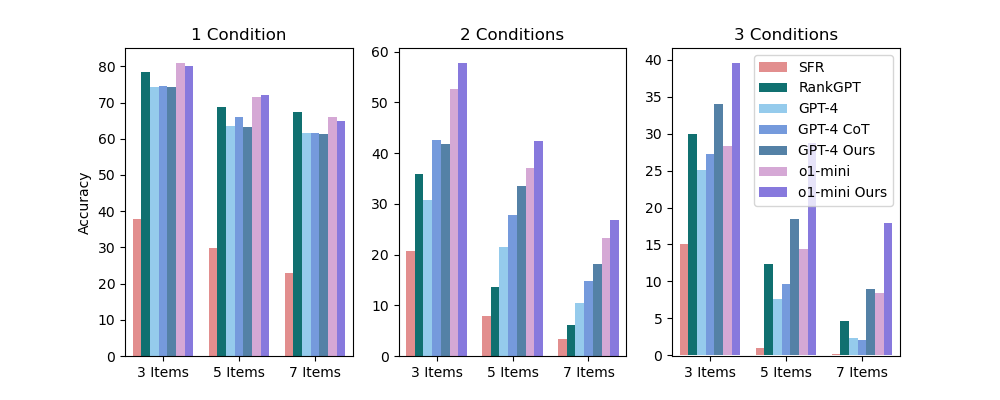
\includegraphics[width=\linewidth]{submissions/Estevam2024/figures/new_token-bar.png}
    \vskip -1.8mm
    \caption{Evaluating the impact of EXSIR against zero-shot CoT prompting for token-level items. We additionally report SFR and RankGPT performances as representatives of existing rankers.}
    \label{fig:tok-bar}
\end{figure*}

\subsubsection{Trust but Verify}
Motivated by the observations from the study reported in Section~\ref{sec:rag_accountable},
we create a two-stage review-then-rationalize (see Figure~\ref{fig:acc-rationalizer}) pipeline to evaluate the impact of intervening  
incorrect model predictions before rationalization. 
The pipeline instruments a \emph{reviewer} module
that employs another LLM (GPT-3.5 \code{text-davinci-003} (\code{temperature = 0})) to evaluate the correctness
of the knowledge-intensive task (KIT) model and refrain from
rationalizing potentially incorrect decisions. 
\begin{figure}[!htb]
    \centering
    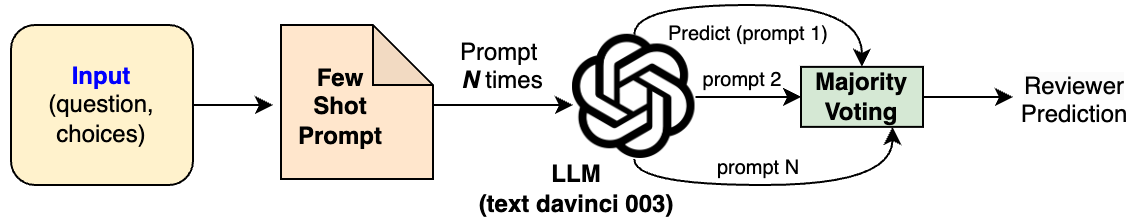
\includegraphics[width=0.7\linewidth]{submissions/Estevam2024/figures/block-accountable.drawio.png}
    \caption{Self-consistency-based Reviewer---intervene for any disagreement with the KIT model prediction.}
    \label{fig:acc-rationalizer}
\end{figure}
 
Depending on the task and data domain, the suitability of the reviewer model may vary. Given the complexity of knowledge-intensive tasks, 
 we employ a self-consistency-based decoding strategy~\cite{wang2022self} where the reviewer is asked the same question $N$ (=5) times, and the final response is selected via majority voting. The reviewer then compares the model's prediction with its prediction, and The rationalizer is utilized only when the KIT model and the reviewer agree. 

 \begin{table}[!htb]
\scriptsize
\centering
\begin{tabular}{cccc}
\hline
\multicolumn{1}{c}{\multirow{2}{*}{\textbf{Dataset}}} & \multicolumn{1}{c}{\textbf{Prediction Errors}} & \multicolumn{2}{c}{\textbf{Errors Intervened}}                                                \\ \cline{3-4} 
\multicolumn{1}{c}{}                                  & \multicolumn{1}{c}{\textbf{(Test Set)}}        & \multicolumn{1}{c}{\textbf{Greedy Decoding}} & \multicolumn{1}{c}{\textbf{Self-consistency}} \\ \hline
CSQA                                                    & 321                                             & \multicolumn{1}{c}{166 ($51.71\%$)}                     & 187 ($\mathbf{58.26\%}$)                                        \\ %\hline
OBQA                                                    & 155                                             & \multicolumn{1}{c}{102 ($65.81\%$)}                     & 110 ($\mathbf{70.97\%}$)                                         \\ \hline
\end{tabular}
\caption{The review-then-rationalize pipeline helps intervene in incorrect predictions of a knowledge-intensive task (KIT) model. The self-consistency-based reviewer outperforms the greedy decoding-based reviewer.}
\label{tab:review}
\end{table}

As shown in Table~\ref{tab:review}, for knowledge-intensive tasks such as Commonsense QA and Openbook QA, the proposed pipeline helps intervene up to $58\%$ and $71\%$ of the incorrect predictions. Unsurprisingly, the self-consistency-based reviewer outperforms the greedy decoding-based reviewer. Overall, \emph{the results draw attention to the importance of responsibly communicating LLM-generated rationales to humans and, consequently, instrumenting guardrails as an effective intervention strategy.} 

\subsection{Orchestration Under Real-World Constraints}
\label{sec:blue-orchestration}
In real-world applications, RAG systems must operate under various constraints such as processing time, resource limitations, and compliance requirements. Efficient orchestration of RAG pipelines, involving the coordination of multiple processes (retrieval, generation, and post-processing), can be challenging but offers unique advantages.
%
We propose a blueprint architecture~\cite{kandogan2024blueprint} where the key orchestration concept is ``streams'' to coordinate the flow of data and instructions among components of varying compute requirements.



Key components in the blueprint architecture include (Figure~\ref{fig:architecture}): (1) \emph{agents, agent and data registries} as key touch points and interfaces to seamlessly integrate with existing deployed models, APIs, databases, and services, (2) \emph{streams} to orchestrate data and instructions across components, and (3) \emph{task and data planners} to optimize for cost and quality constraints in task execution and data retrieval.
%
It is designed for seamless integration into existing infrastructure, enabling extensibility, customizability, and reusability through well-defined touchpoints and interfaces. It supports externalized orchestration and flexible task coordination via declarative plans, ensuring observability, controllability, and optimized performance while meeting quality-of-service constraints.



\begin{figure}[!htb] 
  \vspace{-10pt}
  \centering
  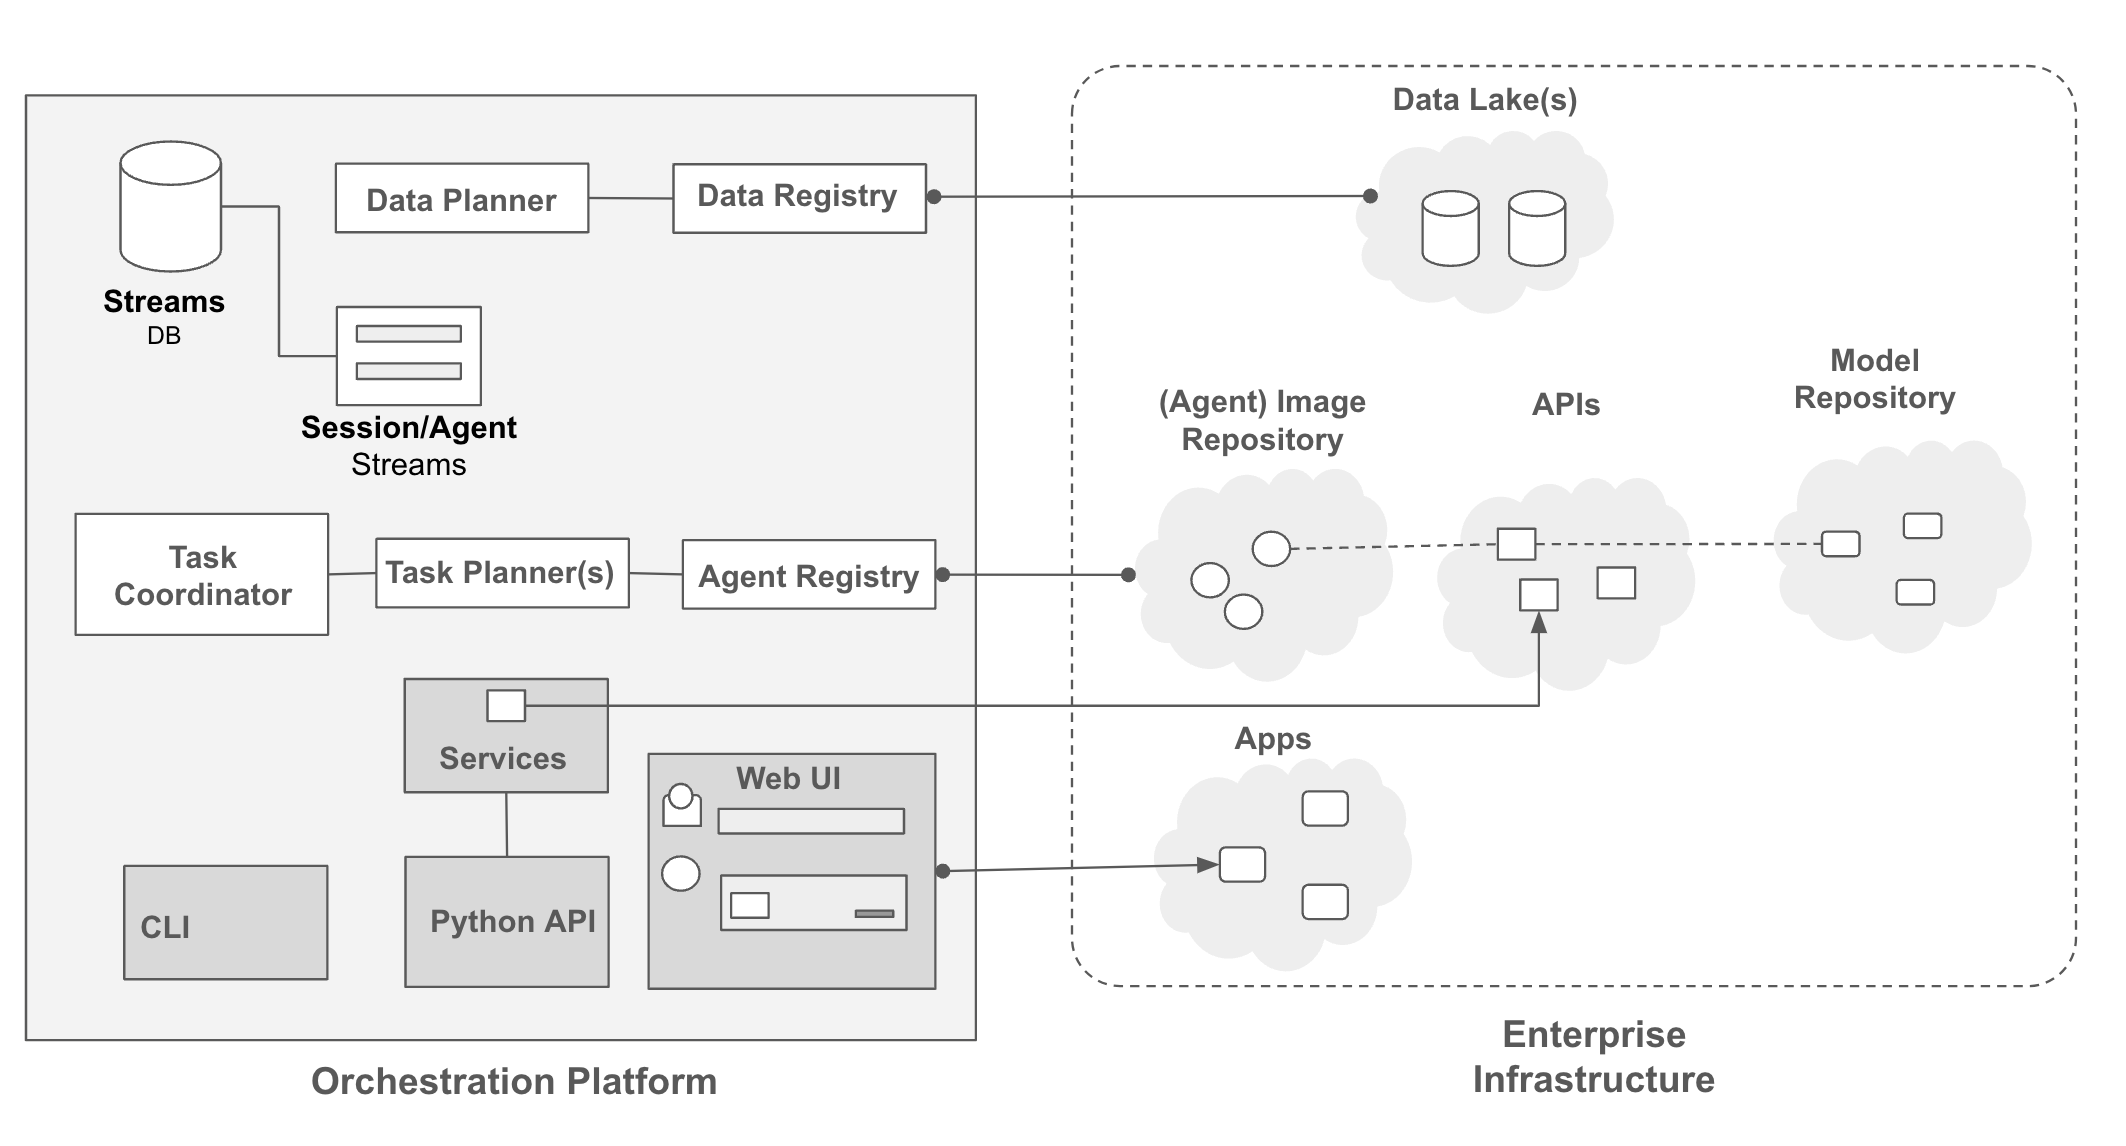
\includegraphics[width=\linewidth]{submissions/Estevam2024/figures/architecture.png}
  \caption{Blueprint Architecture: Data and Agent Registries are touch points that define existing data, models, APIs, and services in the enterprise for utilization by agents.}
  \label{fig:architecture} 
  \vspace{-15pt}
\end{figure}

\section{Challenges and Opportunities}
\label{sec:future}
The work discussed covers limited aspects of building an effective System 2 RAG solution. Numerous intriguing research questions remain unanswered in the fields of NLP, AI, databases, and HCI, presenting ample opportunities for interdisciplinary collaboration. Here, we will discuss some of these questions.
\subsection{Planning and reasoning}
Despite emerging attempts to explore LLMs' reasoning capabilities and use them as planners~\cite{zhao2024large, huang2022language} or `routers' of existing tools and APIs~\cite{liang2024taskmatrix, qin2023toolllm,kim2023llmcompiler}, LLMs alone still cannot solve the planning problem~\cite{kambhampati2024llms,valmeekam2023planning}. Key questions remain, including: How to exploit LLMs for planning, yet add verification and constraints? How to perform planning over multi-modal (relational, graph, documents, parametric) data sources?
How to interact with the user in regards to planning, present and refine plans collaboratively? How to learn feedback and attribute back to agents and operators?


In addition, Optimization is critical for planning for production both as a driver of QoS and business-wise, as cost and performance affect the bottom line. Optimization is a well-studied subject, but new questions emerge: How to perform cost estimation for (new) agents, given the dependence on data (size and beyond)? How to handle uncertainty in sources such as LLMs? How to estimate the overall plan cost? How to incorporate an accrued budget into planners?

Additional future research opportunities in reasoning and decision-making systems exist in addressing the overhead introduced by deliberate, system 2 thinking processes, such as planning, which can be slow and cause notable differences in enterprise setups. A promising direction involves alleviating this burden by moving parts of the system 2 thinking process offline, continuously distilling and materializing knowledge into diverse representations. Metaphorically, this is akin to learning to drive: while initial skill acquisition requires deliberate system 2 reasoning, skilled drivers rely on system 1 instincts, reacting fluidly without explicitly thinking about each action, as their expertise becomes ingrained like muscle memory. Similarly, RAG systems can benefit significantly from insights derived from both online and offline learning processes. These insights can extend beyond traditional model weights to include artifacts like graphs, tables, and natural language documents. This calls for research in areas such as knowledge distillation, insight extraction, and planning, with a focus on understanding when and where to trust instinctual, system 1 insights versus when to engage in more rigorous, system 2 reasoning.
\subsection{Multi-modal data}
Enterprise environments often contain highly varied data sources, including databases, document collections, graphs, and structured tables with heterogeneous schemas. RAG systems designed for these environments must be capable of handling data from diverse formats while preserving contextual coherence across data types. They face challenges ranging from architectural and representational choices to managing ambiguity and uncertainty across modalities. How can RAG models balance capturing detailed, structured knowledge from tables or graphs with synthesizing general information from unstructured text? How should confidence levels and uncertainty be managed when retrieving from different data types? And how should the relevance of retrieved information be measured when dealing with multiple data types, given that existing metrics are often optimized for text-based retrieval?

\subsection{From Data to Insights}
A core opportunity in RAG systems lies in their ability to transform raw data into actionable insights. This insight-driven retrieval allows systems to dynamically generate responses tailored to user-specific needs or industry contexts. For example, RAG systems in human resources might leverage real-time job market statistics to enhance job recommendations, improving matches based on current industry trends. By deriving insights, systems can synthesize contextual knowledge from data, supporting more accurate and adaptive output generation.

However, research challenges remain. For instance, how can RAG systems accurately capture and prioritize real-time, evolving information from different data sources to ensure that insights remain relevant and current? In dynamic fields such as job searching, the timeliness and accuracy of insights can be critical. Moreover, what methods can be developed to quantify and communicate the reliability or confidence level of synthesized insights to end users? Trustworthiness becomes especially important when RAG systems support high-stakes decision-making.
%\subsection{Agentic Workflows}

\section{Conclusion}

In this work, we explored the limitations of current Retrieval-Augmented Generation (RAG) models and proposed that a System 2 perspective should be adopted to address the challenges faced by LLMs in complex, domain-specific enterprise applications. Despite the advancements in integrating external information for grounding LLM outputs, we highlighted the shortcomings of existing RAG approaches, which often lack rigorous reasoning and deliberative analytics characteristic of System 2 thinking. Our analysis is based on the literature review and results obtained in previous work on different aspects of LLMs limitations and current RAG approaches, and it reinforces the necessity of transitioning from monolithic LLM architectures to compound AI systems, which employ specialized agents to enhance retrieval, ensure factual correctness, and mitigate issues like hallucination.

Based on the results already obtained by the previously described approaches that incorporate initial steps towards the System 2 type of thinking, we outlined a vision for the future, emphasizing the design of compound systems that better align with System 2 principles, featuring coordinated, logic-driven workflows capable of holistic reasoning and cross-document synthesis. While our work provides a foundational perspective for these advancements, there are still open questions about optimizing retrieval strategies, seamlessly integrating multiple data types, and fine-tuning decision-making modules. Addressing these challenges will be crucial for deploying robust, trustworthy AI systems that meet the high standards of reliability and precision required in enterprise contexts.







\section*{Acknowledgment}

We thank the Editors of IEEE Data Engineering Bulletin for their valuable feedback: their suggestions immensely improved the quality of the article. Exploring these research problems required a significantly larger cast of characters than the author list in this paper does justice. We thank the co-authors of all the research papers cited in this article. 



\bibliographystyle{IEEEtran}
\bibliography{submissions/Estevam2024/custom,submissions/Estevam2024/custom_dz}

% \begin{thebibliography}{00}
% \bibitem{b1} G. Eason, B. Noble, and I. N. Sneddon, ``On certain integrals of Lipschitz-Hankel type involving products of Bessel functions,'' Phil. Trans. Roy. Soc. London, vol. A247, pp. 529--551, April 1955.
% \bibitem{b2} J. Clerk Maxwell, A Treatise on Electricity and Magnetism, 3rd ed., vol. 2. Oxford: Clarendon, 1892, pp.68--73.
% \bibitem{b3} I. S. Jacobs and C. P. Bean, ``Fine particles, thin films and exchange anisotropy,'' in Magnetism, vol. III, G. T. Rado and H. Suhl, Eds. New York: Academic, 1963, pp. 271--350.
% \bibitem{b4} K. Elissa, ``Title of paper if known,'' unpublished.
% \bibitem{b5} R. Nicole, ``Title of paper with only first word capitalized,'' J. Name Stand. Abbrev., in press.
% \bibitem{b6} Y. Yorozu, M. Hirano, K. Oka, and Y. Tagawa, ``Electron spectroscopy studies on magneto-optical media and plastic substrate interface,'' IEEE Transl. J. Magn. Japan, vol. 2, pp. 740--741, August 1987 [Digests 9th Annual Conf. Magnetics Japan, p. 301, 1982].
% \bibitem{b7} M. Young, The Technical Writer's Handbook. Mill Valley, CA: University Science, 1989.
% \end{thebibliography}

\end{document}
